\documentclass[11pt, a4paper]{article}

\usepackage[utf8]{inputenc}
\usepackage{fullpage}
\usepackage[parfill]{parskip} % Empty line instead of indentation
\usepackage{graphicx}
\graphicspath{ {images/} }
\usepackage{color}
\usepackage{tabularx}
\usepackage{listings}
\usepackage{caption}
\usepackage{subcaption}
\usepackage{mathtools}
\usepackage{amssymb}
\usepackage{eurosym}
\usepackage[ngerman]{babel}
\usepackage[normalem]{ulem} %Squiggly underline
\usepackage{cancel} %Kürzen

\newcommand\braces[1]{\left(#1\right)}
\newcommand\brackets[1]{\left[#1\right]}
\renewcommand{\vec}[1]{\underline{#1}}
\newcommand{\mat}[1]{\underline{\underline{#1}}}
\newcommand{\abs}[1]{\left\lvert#1\right\rvert}
\newcommand{\norm}[1]{\left\lVert#1\right\rVert}
\newcommand\tr[1]{\mathrm{tr}\br{#1}}
\newcommand\average[1]{\left\langle#1\right\rangle}
\newcommand{\acos}[1]{\mathrm{acos}\braces{#1}}
\newcommand{\asin}[1]{\mathrm{asin}\braces{#1}}
\newcommand{\intend}[1][]{\ \mathrm{d}#1}
\newcommand{\derivative}[2][]{\ \frac{\mathrm{d}#1}{\mathrm{d}#2}} %\derivative[a]{b}
\newcommand\expectedValue[1]{\mathbb{E}\braces{#1}}
\newcommand\variance[1]{\mathbb{V}\braces{#1}}
\newcommand\setequal{\overset{!}{=}}
\newcommand{\gerquote}[1]{\glqq#1\grqq}

\lstset{
	tabsize=4,
	breaklines=true,
	showspaces=false,
	showstringspaces=false
}

% Set showsolution to false to generate a file that just contains the exercises
% Otherwise, solutions will be included.
\newif\ifshowsolution
\showsolutiontrue
%\showsolutionfalse

\ifshowsolution
	\title{Tutorium WS 15/16 \\ Lösungen}
\else
	\title{Tutorium WS 15/16 \\ Aufgaben}
\fi
\author{Christian Mielers}
\date{\today}

\begin{document}
\maketitle
\tableofcontents

%%%%%%%%%%%%%%%%%%%%%%%%%%%%%%%%%%%%%%%%%%%%%%%%%%%%%%%%%%%%%%%%%%%%%%%%%%%%%%%%
%                                   HöMa                                       %
%%%%%%%%%%%%%%%%%%%%%%%%%%%%%%%%%%%%%%%%%%%%%%%%%%%%%%%%%%%%%%%%%%%%%%%%%%%%%%%%
\newpage
\section{Höhere Mathematik}
\subsection{Wahrheitstabellen}
Prüfe, ob folgende Aussagen gelten

\begin{enumerate}
	\item $(a \lor b) \lor (a \land b) \Leftrightarrow (a \lor b)$
	
	\ifshowsolution
		\begin{tabular}{|c|c||c|c|c||c|}
			\hline
			a & b & $a \lor b$ & $a \land b$ & $(a \lor b) \lor (a \land b)$ & Gesammtterm \vphantom{\Big(}\\
			\hline
			0 & 0 & 0 & 0 & 0 & 1 \\
			0 & 1 & 1 & 0 & 1 & 1 \\
			1 & 0 & 1 & 0 & 1 & 1 \\
			1 & 1 & 1 & 1 & 1 & 1 \\
		   \hline
		\end{tabular}
	\fi

	\item $(a \lor b) \land (a \lor \lnot b) \Leftrightarrow a \lor (b \land \lnot a)$

	\ifshowsolution
		\begin{tabular}{|c|c||c|c|c||c|c||c|}
			\hline
			a & b & $a \lor b$ & $a \lor \lnot b$ & $(a \lor b) \land (a \lor \lnot b)$ &
			$b \land \lnot a$ & $a \lor (b \land \lnot a)$ & Gesammtterm \vphantom{\Big(} \\
			\hline
			0 & 0 & 0 & 1 & 0 & 0 & 0 & 1 \\
			0 & 1 & 1 & 0 & 0 & 1 & 1 & 0 \\
			1 & 0 & 1 & 1 & 1 & 0 & 1 & 1 \\
			1 & 1 & 1 & 1 & 1 & 0 & 1 & 1 \\
		  \hline
		\end{tabular}
	\fi

	\item $\left((a \lor b) \Rightarrow (a \land b) \right) \Leftrightarrow (a \land b) \lor (\lnot a \land \lnot b)$

	\ifshowsolution
		\begin{tabular}{|c|c||c|c|c||c|c||c|}
			\hline
			a & b & $a \lor b$ & $a \land b$ & $(a \lor b) \Rightarrow (a \land b)$ &
			$(a \land b) \lor (\lnot a \land \lnot b)$ & $\lnot a \land \lnot b$ & Gesammtterm \vphantom{\Big(} \\
			\hline
			0 & 0 & 0 & 0 & 1 & 1 & 1 & 1 \\
			0 & 1 & 1 & 0 & 0 & 0 & 0 & 1 \\
			1 & 0 & 1 & 0 & 0 & 0 & 0 & 1 \\
			1 & 1 & 1 & 1 & 1 & 1 & 0 & 1 \\
		  \hline
		\end{tabular}
	\fi
\end{enumerate}

\subsection{Mengenlehre}
Gelten die folgenden Beziehungen für beliebige Mengen X, Y und Z?
\begin{enumerate}
	\item $X \setminus (Y \cap Z) = (X \setminus Y) \cap (X \setminus Z)$
	
	\ifshowsolution
		\begin{figure}[h!]
			\centering
			\begin{subfigure}{3cm}
				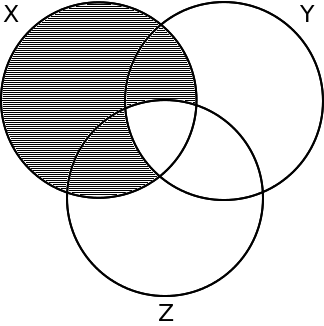
\includegraphics[height=3cm]{MengenlehreAufgabe1a}
				\caption{Linke Seite}
			\end{subfigure}
			\hspace{2cm}
			\begin{subfigure}{3cm}
				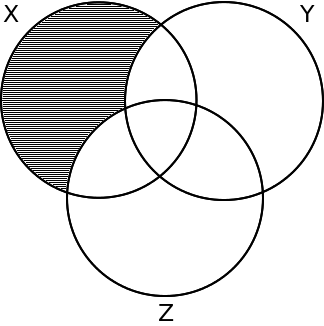
\includegraphics[height=3cm]{MengenlehreAufgabe1b}
				\caption{Rechte Seite}
			\end{subfigure}
		\end{figure}
	
		Gegenbeispiel finden: $X \cup Y$ oder $X \cup Z$ darf nicht leer sein. \\
		Sei $X = \{1,2,3\}, Y = \{2,4,6\}$ und $Z = \{7,8,9\}$ \\
		Dann ist $X \setminus (Y \cap Z) = \{1,2,3\} \quad \neq \quad \{1,3\} = (X \setminus Y) \cap (X \setminus Z)$
	\fi
	
	\item $(X \cup Y) \setminus Z = \Big((X \setminus Z) \cup (Y \setminus Z)\Big) \setminus (Y \cap Z)$
	
	\ifshowsolution
		\begin{figure}[h!]
			\centering
			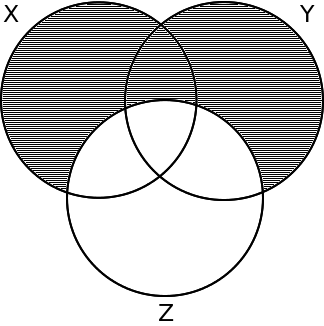
\includegraphics[height=3cm]{MengenlehreAufgabe2}
			\caption{linke / rechte Seite}
		\end{figure}
		
		\begin{align*}
			(X \cup Y) \setminus Z &= \Big((X \setminus Z) \cup (Y \setminus Z)\Big) \setminus (Y \cap Z) \\
			(X \cup Y) \setminus Z &= \Big( (X \cup Y) \setminus Z \Big) \setminus (Y \cap Z) \\
			(X \setminus Z) \cup (Y \setminus Z) &= (X \setminus Z) \cup (Y \setminus Z)
		\end{align*}
	\fi
	
	\item $X \cup (Y \cap Z) = (X \cup Y) \cap (X \cup Z)$
	\ifshowsolution
		\begin{figure}[h!]
			\centering
			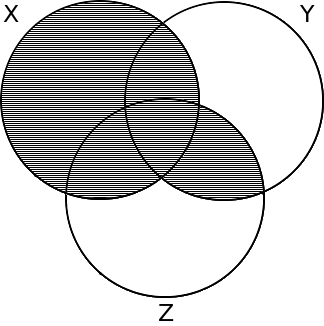
\includegraphics[height=3cm]{MengenlehreAufgabe3}
			\caption{linke / rechte Seite}
		\end{figure}
	
		\begin{align*}
			X \cup (Y \cap Z) &= (X \cup Y) \cap (X \cup Z) \\
			X \cup (Y \cap Z) &= X \cup (Y \cap Z) \tag{Distributivitätsgesetz}
		\end{align*}
	\fi
\end{enumerate}

\subsection{Abbildungen}
Sind die folgenden Funktionen injektiv, surjektiv, bijektiv?
\begin{enumerate}
	\item $\mathrm{f}(x) = x^4+2 \qquad \mathrm{f}: \mathrm{R} \mapsto \mathrm{R}$
	
	\ifshowsolution
		nicht injektiv: $\mathrm{f}(1) = \mathrm{f}(-1)$ \\
		nicht surjektiv: $\forall x: \mathrm{f}(x) \geq 2$. Alternativ: $\nexists x: \mathrm{f}(x) = 0$ \\
		Somit ist f nicht bijektiv.
	\fi
	
	\item $\mathrm{f}(x) = x^4+2 \qquad \mathrm{f}: \mathrm{R} \mapsto (2, + \infty)$
	\ifshowsolution
		nicht injektiv: $\mathrm{f}(1) = \mathrm{f}(-1)$ \\
		surjektiv: $\mathrm{f}(x) = x^4 + 2 \Leftrightarrow \sqrt[4]{\mathrm{f}(x) - 2} = x$ \\
		$\sqrt[4]{\mathrm{f(x)}-2}$ existiert eindeutig für $x \geq 2$ (und somit auch für $x > 0$) \\
		Somit ist f nicht bijektiv.
	\fi
	
	\item $\mathrm{f}(x) = x^3+1 \qquad \mathrm{f}: \mathrm{R} \mapsto \mathrm{R}$
	
	\ifshowsolution
		injektiv: $x^3 + 1 = y^3 + 1 \Rightarrow x^3 = y^3 \Rightarrow x = y$ (Technischer: $\nexists x \neq y: x^3 + 1 \neq x^3 + 1$) \\
		surjektiv: $\forall y \in \mathrm{R}: \exists x \in \mathrm{R}: y = x^3 + 1 \Leftrightarrow y - 1 = x^3 \Leftrightarrow \sqrt[3]{y-1} = x$
		Somist ist f bijektiv.
	\fi
	
	\item $\mathrm{f}(x) = \sin(x) \qquad \mathrm{f}: \mathrm{R} \mapsto [-1, 1]$
	
	\ifshowsolution
		nicht injektiv: $\sin(\pi) = \sin(2 \pi)$ \\
		surjektiv: $\sin \braces{-\frac{\pi}{2}} = -1$, $\sin \braces{\frac{\pi}{2}} = 1$ und $\sin(x)$ steigt auf dem stetigen Intervall $\brackets{-\frac{\pi}{2},-\frac{\pi}{2}}$ monoton. \\
		Somit ist f nicht bijektiv.
	\fi
	
	\item $\mathrm{f}(x) = x^4 - x^2 \qquad \mathrm{f}: \mathrm{R} \mapsto \mathrm{R}$
	
	\ifshowsolution
		nicht injektiv: $\mathrm{f}(1) = \mathrm{f}(-1)$ \\
		nicht surjektiv: $\nexists x: \mathrm{f}(x) = 0$ \\
		Somit ist f nicht bijektiv.
	\fi
	
	\item $\mathrm{f}(x) = \frac{1}{x} \qquad \mathrm{f}: \mathrm{R} \mapsto \mathrm{R}$
	
	\ifshowsolution
		injektiv: Sei $x \neq y$. Dann $\frac{1}{x} \neq \frac{1}{x}$ \\
		nicht surjektiv: $\nexists x \in \mathrm{R}: \frac{1}{x} = 0$ \\
		Somit ist f nicht bijektiv.
	\fi
\end{enumerate}

Invertiere folgende Funktionen:

Zum invertieren tausche x und f(x) bzw. x und y und löse nach f(x) bzw. y auf. Bei Schrittweise definierten Funktionen müssen auch die Grenzen angepasst werden!
\begin{enumerate}
	\item $\mathrm{f}(x) = x^3 \qquad \mathrm{f}: \mathrm{R} \mapsto \mathrm{R}$
	
	\ifshowsolution
		$x = {\mathrm{f}(x)}^3$ \\
		$\sqrt[3]{x} = f(x)$
	\fi
	
	\item $\mathrm{f}(x) = \frac{1}{x} \qquad \mathrm{f}: \mathrm{R} \setminus \{0\} \mapsto \mathrm{R} \setminus \{0\}$
	
	\ifshowsolution
		$x = \frac{1}{\mathrm{f}(x)}$ (Vertauschen von f(x) und x)\\
		$\mathrm{f}(x) = \frac{1}{x}$ (Aufgelöst nach f(x))
	\fi
	
	\item $\mathrm{f}(x) =
		\begin{cases}
			-\frac{1}{2}x + 3 & x \in (-\infty, 4) \\
			-3x + 13 & x \in [4, +\infty)
		\end{cases}
		$
		
	\ifshowsolution
		\begin{enumerate}
			\item $\mathrm{f}(x) = -\frac{1}{2}x + 3$ invertieren \\
				\begin{align*}
					x &= -\frac{1}{2}\mathrm{f}(x) + 3 \\
					x-3 &= -\frac{1}{2}\mathrm{f}(x) \\
					-2x+6 &= \mathrm{f}(x)
				\end{align*}
			\item $\mathrm{f}(x) = -3x + 13$ invertieren
			\begin{align*}
				x = -3 \mathrm{f}(x) + 13 \\
				x - 13 = -3 \mathrm{f}(x) \\
				\frac{-x + 13}{3} = \mathrm{f}(x)
			\end{align*}
			\item Grenzen neu berechnen \\
			y-Wert des Schnittpunktes in Umkehrfunktion der Funktion einsetzen, die den Schnittpunkt enthält: \\
			$\mathrm{f}(1) = \frac{-1 + 13}{3} = 4$ \\
			Der neue Schnittpunkt hat also die Koordinaten (1,4)
		\end{enumerate}
		Die Umkehrfunktion ist somit:
		$\begin{cases}
			-2x+6, & x \in (-\infty,1) \\
			\frac{-x + 13}{3} & x \in [1, +\infty)
		\end{cases}$
	\fi
\end{enumerate}

\subsection{Algebraische Strukturen}
Eine Algebraische Struktur kann (u.A.) folgende Eigenschaften aufweisen:
\begin{description}
	\item[A1] Assoziativität (Addition)
	\item[A2] Kommutativität (Addition)
	\item[A3] Neutrales Element (Addition)
	\item[A4] Inverses Element (Addition)
	\item[M1] Assoziativität (Multiplikation)
	\item[M2] Kommutativität (Multiplikation)
	\item[M3] Neutrales Element (Multiplikation)
	\item[M4] Inverses Element (Multiplikation)
	\item[D] Distributivität
\end{description}
Sind A1 - A4 erfüllt handelt es sich um eine Kommutative Gruppe, bei A1-M2 und D um einen Kommutativen Ring und ein Körper ist die Struktur dann, wenn alle Eigenschaften erfüllt sind.

Sind folgende Mengen-Abbildungspaare Gruppen, Ringe, Körper oder nichts davon?

\begin{enumerate}
	\item $\braces{\mathbb{N}_0, +}$
	
	\ifshowsolution
		$\braces{\mathbb{N}_0, +}$ ist nichts von dem, da kein inverses Element bzgl. +: $\nexists x \in \mathbb{N}_0: 3+x=0$
	\fi
	
	\item $\braces{\mathbb{Z}, +}$ \label{ZGruppe}
	
	\ifshowsolution
		Addition ist Assoziativ \\
		Addition ist Kommutativ \\
		0 ist das neutrale Element der Addition und $0 \in \mathbb{Z}$ \\
		Das inverse Element zu a ist $-a$
		$\braces{\mathbb{Z}, +}$ ist somit eine Gruppe
	\fi
	
	\item $\braces{\mathbb{Z}, +, \cdot}$
	
	\ifshowsolution
		Axiome für die Addition gelten (siehe \ref{ZGruppe}.) \\
		Multiplikation ist Assoziativ: $(a \cdot b) \cdot c = a \cdot (b \cdot c)$ \\
		Multiplikation ist Kommutativ: $a \cdot b = b \cdot a$ \\
		Das Distributivgesetzt gilt für Addition und Multiplikation: $a(b+c) = ab + ac$ \\
		$\braces{\mathbb{Z}, +, \cdot}$ ist somit ein Ring. \\ \\
		Aber: $\braces{\mathbb{Z}, +, \cdot}$ ist kein Körper! \\
		Es gibt zwar ein neutrales Element der Multiplikation (die 1), aber es gibt nicht für jedes Element eine Inverse, für die 3 z.B. nicht: $\nexists x \in \mathbb{Z}: 3\cdot x = 1$
	\fi
	
	\item $\braces{\mathbb{R}, +, \cdot}$
	
	\ifshowsolution
		Axiome für Addition gelten (siehe \ref{ZGruppe}.) \\
		Assoziativität und Kommutativität der Multiplikation gelten (siehe \ref{ZRing}.) \\
		Distributivität gilt (siehe \ref{ZRing}.) \\
		1 ist das neutrale Element der Multiplikation. \\
		Das inverse Element zu a ist $\frac{1}{a}$ (und jeder Bruch ist $\in \mathbb{R}$). \\
		$\braces{\mathbb{R}, +, \cdot}$ ist somit ein Körper.
	\fi
	
	\item $\braces{\mathrm{M}, +, \cdot}$ mit $\mathrm{M} = \{ -2,0,\frac{1
	}{2},1,2 \}$
	
	\ifshowsolution
		Verletzung der Abgeschlossenheit: $1+2 \notin \mathrm{M}$, somit gilt nicht: $\mathrm{M} \times \mathrm{M} \mapsto \mathrm{M}$ \\
		Kein additives Inverses zu 1: $\nexists x \in \mathrm{M}: 1+x=0$ \\
		Kein multiplikatives Inverses zu -2: $\nexists x \in \mathrm{M}: -2 \cdot x = 1$ \\
		$\braces{\mathrm{M}, +, \cdot}$ mit $\mathrm{M} = \{ -2,0,\frac{1
	}{2},1,2 \}$ ist somit nichts von alledem.
	\fi
	
	\item $\braces{\mathbb{R}, +, \circ}$ mit $a \circ b = 3a + b$
	
	\ifshowsolution
		$\circ$ ist nicht assoziativ:
		\begin{align*}
			(a \circ b) \circ c &= a \circ (b \circ c) \\
			(3a + b) \circ c &= a \circ (3b + c) \\
			3(3a + b) + c &= 3a + (3b + c) \\
			9a &\neq 3a
		\end{align*}
		
		Somit ist $\braces{\mathbb{R}, +, \circ}$ mit $a \circ b = 3a + b$ nichts von alledem.
	\fi
\end{enumerate}

\subsubsection{Kommutative Gruppen}
Zeige, dass $(G,\circ)$ mit $G=\mathbb{R} \setminus \{1\}$ und $x \circ y = x+y-xy$ eine kommutative Gruppe ist. Was ist das neutrale Element, und wie bildet sich das inverse Element?

\ifshowsolution
	\begin{enumerate}
		\item[(A1)] $(x \circ y) \circ z = x \circ (y \circ z)$
			\begin{align*}
				(x+y-xy) \circ z &= x \circ (y+z-yz) \\
				x+y-xy + z - z(x+y-xy) &= x+ y+z-yz - x(y+z-yz) \tag*{$-x-y-z$} \\
				-xy - (zx+zy-xyz)&= -yz - (xy+xz-xyz) \\
				-xy - zx - zy + xyz &= -yz - xy - xz + xyz \tag*{- xyz + xy} \\
				- zx - zy &= -yz - xz \tag*{sichtbar gleich}
			\end{align*}
		\item[(A2)] $x \circ y = y \circ x$
			\begin{align*}
				x+y-xy &= y+x-xy \\
				x+y-xy &= x+y-xy
			\end{align*}
		\item[(A3)] $"0" \circ x = x$ (neutrales Element, hier n)
			\begin{align*}
				n \circ x &= x \\
				n+x-nx &= x \\
				\underbrace{(1-n)}_{=1}x &= x \\
				n &= 0
			\end{align*}
		\item[(A4)] $x \circ (-x) = 0$ bzw. $x \circ i = n$
			\begin{align*}
				x + i - xi &= 0 \\
				i - xi &= -x \\
				(1-x)i &= -x \\
				i &= \frac{-x}{1-x} \tag*{$1 \notin G$} \\
				i &= \frac{x}{x-1}
			\end{align*}
	\end{enumerate}
\fi

\subsubsection{Körper}
Vervollständige folgende Tabellen für den Körper $K = \left\{\{0,1,a,b,c\right\}, +, \cdot\} $. 0 ist das neutrale Element der Addition, 1 der Multiplikation

Was ist das inverse Element von b in K bzgl. der Multiplikation?

\ifshowsolution
	\begin{center}
		\begin{tabular}{c|ccccc}
			+ & 0 & 1 & a & b & c \\ \hline
			0 & 0 & 1 & a & b & c \\
			1 & 1 & a & b & c & 0 \\
			a & a & b & c & 0 & 1 \\
			b & b & c & 0 & 1 & a \\
			c & c & 0 & 1 & a & b \\
		\end{tabular}
		\hspace{2cm}
		\begin{tabular}{c|ccccc}
			$\cdot$ & 0 & 1 & a & b & c \\ \hline
			0 & 0 & 0 & 0 & 0 & 0 \\
			1 & 0 & 1 & a & b & c \\
			a & 0 & a & c & 1 & b \\
			b & 0 & b & 1 & c & a \\
			c & 0 & c & b & a & 1 \\
		\end{tabular}
	\end{center}
	$a \equiv 2, \quad b \equiv 3, \quad c \equiv 4$

	Finde x so dass $a \cdot b \cdot x = a$ bzw. $b \cdot x = 1$. Die Inverse von $b$ ist also a: $b^{-1} = a$
\else
	\begin{center}
	\begin{tabular}{c|ccccc}
		+ & 0 & 1 & a & b & c \\ \hline
		0 &  &  &  &  & \\
		1 &  &  &  &  & \\
		a &  &  &  &  & \\
		b &  &  &  &  & \\
		c &  & 0 & 1 &  & \\
	\end{tabular}
	\hspace{2cm}
	\begin{tabular}{c|ccccc}
		$\cdot$ & 0 & 1 & a & b & c \\ \hline
		0 &  &  &  &  & \\
		1 &  &  &  &  & \\
		a &  &  &  &  & \\
		b &  &  &  &  & \\
		c &  &  &  &  & \\
	\end{tabular}
\end{center}
\fi

\ifshowsolution
	\begin{center}
		\begin{tabular}{c|ccccc}
			+ & 0 & 1 & a & b & c \\ \hline
			0 & 0 & 1 & a & b & c \\
			1 & 1 & b & 0 & c & a \\
			a & a & 0 & c & 1 & b \\
			b & b & c & 1 & a & 0 \\
			c & c & a & b & 0 & 1 \\
		\end{tabular}
		\hspace{2cm}
		\begin{tabular}{c|ccccc}
			$\cdot$ & 0 & 1 & a & b & c \\ \hline
			0 & 0 & 0 & 0 & 0 & 0 \\
			1 & 0 & 1 & a & b & c \\
			a & 0 & a & 1 & c & b \\
			b & 0 & b & c & a & 1\\
			c & 0 & c & b & 1 & a \\
		\end{tabular}
	\end{center}
	$a \equiv 4, \quad b \equiv 2, \quad c \equiv 3$
\else
	\begin{center}
		\begin{tabular}{c|ccccc}
			+ & 0 & 1 & a & b & c \\ \hline
			0 &  &  &  &  & \\
			1 &  &  &  &  & \\
			a &  & 0 & c &  & \\
			b &  &  &  &  & \\
			c &  &  &  &  & \\
		\end{tabular}
		\hspace{2cm}
		\begin{tabular}{c|ccccc}
			$\cdot$ & 0 & 1 & a & b & c \\ \hline
			0 &  &  &  &  & \\
			1 &  &  &  &  & \\
			a &  &  &  &  & \\
			b &  &  &  &  & \\
			c &  &  &  &  & \\
		\end{tabular}
	\end{center}
\fi

\subsection{Summen und Produkte}
Berechne folgende Summen:
\begin{enumerate}
	\item $\sum_{i=2}^{15} 4$
	
	\ifshowsolution
		$\sum_{i=2}^{15} = 14 \cdot 4 = 56$
	\fi
	
	\item $\sum_{i=0}^5 i^3$
	
	\ifshowsolution
		$\sum_{i=0}^5 i^3 = 0 + 1 + 8 + 27 + 64 + 125 = 225$
	\fi
	
	\item $\sum_{i=0}^5 (-1)^i (4i+3)$
	
	\ifshowsolution
		$\sum_{i=0}^5 (-1)^i (4i+3) = 3-7+11-15+19-23 = -12$
	\fi
\end{enumerate}

Berechne folgende Produkte:
\begin{enumerate}
	\item $\prod_{i=1}^7 i$
	
	\ifshowsolution
		$\prod_{i=1}^7 i = 1 \cdot 2 \dots 6 \cdot 7 = 5040$
	\fi
	
	\item $\prod_{i=1}^4 \frac{i}{2}$
	
	\ifshowsolution
		$\prod_{i=1}^4 \frac{i}{2} = \frac{1}{2} \cdot \frac{2}{2} \cdot \frac{3}{2} \cdot \frac{4}{2} = \frac{24}{2^4} = \frac{3}{2}$
	\fi
	
	\item $\prod_{i=1}^4 \frac{3i^2+2}{i}$
	
	\ifshowsolution
		$\prod_{i=1}^4 \frac{3i^2+2}{i} = \frac{5}{1} \cdot \frac{14}{2} \cdot \frac{29}{3} \cdot \frac{50}{4} = 5 \cdot 7 \cdot \frac{29}{3} \cdot \frac{25}{2} = \frac{25375}{6}$
	\fi
	
\end{enumerate}

\subsection{Binomialkoeffizient}
Für den Binomialkoeffizienten gilt:
$\binom{n}{k} = \frac{n!}{k!(n-k)!}$ \qquad $\binom{n}{n-k} = \binom{n}{k}$ (Symmetrie)

Welchen Wert hat $n$ in den folgenden Gleichungen?
\begin{enumerate}
	\item $ n = \binom{6}{3}$
	
	\ifshowsolution
		$ n = \binom{6}{3} = \frac{6!}{3!(6-3)!} = \frac{\cancel{1\cdot2\cdot3}\cdot4\cdot5\cdot6}{\cancel{(1\cdot2\cdot3)}3!} = \frac{4\cdot5\cdot\cancel{6}}{1\cdot\cancel{2\cdot3}} = 4\cdot5 = 20$
	\fi
	
	\item $n = \binom{10}{7}$
	
	\ifshowsolution
		$n = \binom{10}{7} = \frac{10!}{7!(10-7)!} = \frac{8 \cdot 9 \cdot 10}{3!} = \frac{720}{6} = 120$
	\fi
	
	\item $\binom{n+3}{n+1} + \binom{n+4}{n+2} + \binom{n-1}{n-3} = 70$
	\ifshowsolution
		\begin{align*}
			\binom{n+3}{2} + \binom{n+4}{2} + \binom{n-1}{2} &= 70 \\
			\frac{(n+3)!}{2!(n+3-2)!} + \frac{(n+4)!}{2!(n+4-2)!} + \frac{(n-1)!}{2!(n-1-2)!} &= 70 \tag{Definition} \\
			\frac{(n+3)!}{2(n+1)!} + \frac{(n+4)!}{2(n+2)!} + \frac{(n-1)!}{2(n-3)!} &= 70 \\
			\frac{(n+3)!}{(n+1)!} + \frac{(n+4)!}{(n+2)!} + \frac{(n-1)!}{(n-3)!} &= 140 \tag{Kürzen} \\
			(n+2)(n+3) + (n+3)(n+4) + (n-2)(n-1) &= 140 \\
			n^2+5n+6 + n^2+7n+12 + n^2-3n+2 &= 140 \\
			3n^2+9n-120 &= 0 \\
			n^2+3n-40 &= 0 \tag{PQ-Formel} \\
			x_1 = -8, \quad x_2 &= 5 \tag{Probe!}
		\end{align*}
		Der einfache Binomialkoeffizient ist nur für positive Zahlen definiert, die Lösung ist also $x=1$.
	\fi
\end{enumerate}

\subsection{Ordnungsrelationen}
Ergänze bei folgenden Ausdrücken die Relationszeichen $\subset, \subseteq, \supseteq, \supset,$ oder 'nichts' falls keines davon zutrifft

\ifshowsolution
	\begin{tabular}{|l|c|l|}
		\hline
		Menge 1 & \hspace{3mm} Relation \hspace{3mm} & Menge 2 \\ \hline
		$\{1,2,3\}$ & $\subseteq, \supseteq$ & $\{1,2,3\}$ \\
		$\{5,6\}$ & $\subset$ & $\{5,6,7,8\}$ \\
		$\{\sqrt{2}, \pi, 3\}$ & nichts & $\mathbb{R}$ \\
		$\mathbb{R}$ & $\supset$ & $\mathbb{Q} \setminus {\pi, e}$ \\
		$\mathbb{N}_0$ & $\supset$ & $\mathbb{N}$ \\
		$\mathbb{I}$ & $\subset$ & $\mathbb{R}$ \\
		$\mathbb{C} \setminus \mathbb{I}$ & nichts & $\braces{\mathbb{Q} \setminus \mathbb{N}} \cup \{2,4,6\}$ \\ \hline
	\end{tabular}
\else
	\begin{tabular}{|l|c|l|}
		\hline
		Menge 1 & \hspace{3mm} Relation \hspace{3mm} & Menge 2 \\ \hline
		$\{1,2,3\}$ & & $\{1,2,3\}$ \\
		$\{5,6\}$ & & $\{5,6,7,8\}$ \\
		$\{\sqrt{2}, \pi, 3\}$ & & $\mathbb{R}$ \\
		$\mathbb{R}$ & & $\mathbb{Q} \setminus {\pi, e}$ \\
		$\mathbb{N}_0$ & & $\mathbb{N}$ \\
		$\mathbb{I}$ & & $\mathbb{R}$ \\
		$\mathbb{C} \setminus \mathbb{I}$ & & $\braces{\mathbb{Q} \setminus \mathbb{N}} \cup \{2,4,6\}$ \\ \hline
	\end{tabular}
\fi

\subsection{Ungleichungen}
Für welche Werte von $x$ gelten die folgenden Ungleichungen?
\begin{enumerate}
	\item $5x-3 < \dfrac{2x^2+3x}{x}$
	
	\ifshowsolution
		\begin{align*}
			5x-3 &< 2x+3 \\
			3x &< 6 \\
			x &< 2
		\end{align*}
	\fi
	
	\item $\dfrac{x+1}{2} \geq \abs{2x-3}$
	
	\ifshowsolution
		\begin{align*}
			\dfrac{x+1}{2} &\geq 2 \abs{x-\frac{3}{2}}
			\shortintertext{Fall 1: $x \in \braces{-\infty, \frac{3}{2}}$}
			\dfrac{x+1}{2} &\geq 2 (-1) \braces{x-\frac{3}{2}} \\
			\dfrac{x+1}{2} &\geq 2 \braces{\frac{3}{2} - x} \\
			\dfrac{x+1}{2} &\geq 3 - 2x \\
			x+1 &\geq 6 - 4x \\
			5x &\geq 5 \\
			x &\geq 1
			\intertext{Also Lösung im Fall 1: $x \in \braces{-\infty, \frac{3}{2}} \cap \left[1,+\infty\right) = \left[ 1, \frac{3}{2} \right)$}
			\shortintertext{Fall 2: $x \in \left[ \frac{3}{2}, +\infty \right)$}
			\dfrac{x+1}{2} &\geq 2 \braces{x-\frac{3}{2}} \\
			x+1 &\geq 4x - 6 \\
			7 &\geq 3x \\
			\frac{7}{3} &\geq x
			\intertext{Also Lösung im Fall 2: $x \in \left[ \frac{3}{2}, +\infty \right) \cap \left( -\infty, \frac{7}{3} \right] = \brackets{\frac{3}{2}, \frac{7}{3} }$}
		\end{align*}
		Das Gesammtergebnis ergibt sich also aus $\left[ 1, \frac{3}{2} \right) \cup \brackets{\frac{3}{2}, \frac{7}{3}} = \brackets{1, \frac{7}{3}}$
	\fi
	
	\item $\sqrt{x^2-2x+1} > 3 - \abs{x-2}$
	\ifshowsolution
		\begin{align*}
			\sqrt{(x-1)^2} &> 3 - \abs{x-2} \\
			\abs{x-1} &> 3 - \abs{x-2}
			\shortintertext{Fall 1: $x \in \left( -\infty, 1 \right )$}
			(-1)(x-1) &> 3 + x-2 \\
			1-x &> 3 + x-2 \\
			0 &> 2x \\
			0 &> x
			\intertext{Also Lösung im Fall 1: $x \in \left( -\infty, 1 \right ) \cap \left( -\infty, 0 \right) = \left( -\infty, 0 \right)$}
			\shortintertext{Fall 2: $x \in \left[ 1, 2 \right)$}
			x-1 &> 3 + (x-2) \\
			x > &2 + x \\
			0 &> 2
			\intertext{Also Lösung im Fall 2: $x \in \left[ 1, 2 \right) \cap \emptyset = \emptyset$ (Fall 2 hat keine Lösung!)}
			\shortintertext{Fall 3: $x \in \left[ 2, +\infty \right)$}
			x-1 &> 3 - (x-2) \\
			x-1 &> 3 - x + 2 \\
			2x &> 6 \\
			x &> 3
			\intertext{Also Lösung im Fall 3: $x \in \left[ 2, +\infty \right) \cap \left( 3, +\infty \right) = \left( 3, +\infty \right)$}
		\end{align*}
		Das Gesammtergebnis ergibt sich also aus $\left( -\infty, 0 \right) \cup \left( 3, +\infty \right).$
	\fi
		
	\item $\sqrt{x^2-8x+16} < \frac{\abs{x+2}}{2}$
	\ifshowsolution
		\begin{align*}
			\sqrt{x^2-8x+16} &< \frac{\abs{x+2}}{2} \\
			2 \abs{x-4} &< \abs{x+2}
			\shortintertext{Fall 1: $x \in (-\infty, -2)$}
			2 (-x+4) &< -x-2 \\
			-2x+8 &< -x-2 \\
			10 &< x
			\intertext{Also Lösung im Fall 1: $x \in (10, +\infty) \cap (-\infty, -2) = \emptyset$ (Fall 1 hat keine Lösung!)}
			\shortintertext{Fall 2: $x \in [-2, 4)$}
			2 (-x+4) &< x+2 \\
			-2x+8 &< x+2 \\
			6 &< 3x \\
			2 &< x
			\intertext{Also Lösung im Fall 2: $x \in (2, +\infty) \cap [-2, 4) = (2,4)$}
			\shortintertext{Fall 3: $x \in [4, +\infty]$}
			2 (x-4) &< x+2 \\
			2x-8 &< x+2 \\
			x &< 10
			\intertext{Also Lösung im Fall 3: $x \in (-\infty, 10) \cap [4, +\infty) = [4,10)$}
		\end{align*}
		Das Gesammtergebnis ergibt sich also aus $(2,4) \cup [4,10) = (2,10).$
	\fi
		
	\item $\sqrt{x^2-2x+1} > 3 + \abs{x-2}$
	\ifshowsolution
		\begin{align*}
			\abs{x-1} &> 3 + \abs{x-2} \\
			\abs{x-1} - \abs{x-2} &> 3
		\end{align*}
		Die Ungleichung hat keine Lösung.
	\fi
\end{enumerate}

\subsection{Induktion}
Beweise per vollständiger Induktion:
\begin{enumerate}
	\item $\forall n \geq 1 : \sum_{i=1}^n i = \frac{n(n+1)}{2}$ (Gauß'sche Summenformel)
	
	\ifshowsolution
		\begin{description}
			\item[Anfang] $n=1$
				\begin{align*}
					\sum_{i=1}^1 1 &= \frac{1(1+1)}{2} \\
					1 &= \frac{2}{2}
				\end{align*}
			\item[Annahme] $\sum_{i=1}^n i = \frac{n(n+1)}{2}$
			\item[Schritt] 
			\begin{align*}
				\sum_{i=1}^{n+1} i &= \frac{(n+1)(n+2)}{2} \\
				n+1 + \sum_{i=1}^n i &= \frac{(n+1)(n+2)}{2} \\
				n+1 + \frac{n(n+1)}{2} &= \frac{(n+1)(n+2)}{2} \\
				n+1 + \frac{n^2 + n}{2} &= \frac{n^2 + 3n + 2}{2} \\
				\frac{2n+2}{2} + \frac{n^2 + n}{2} &= \frac{n^2 + 3n + 2}{2} \\
				\frac{n^2 + 3n + 2}{2} &= \frac{n^2 + 3n + 2}{2}
			\end{align*}
		\end{description}
	\fi
	
	\item $\forall n \geq 1 : \sum_{i=1}^n (2i-1) = n^2$ (Summe ungerader Zahlen)
	
	\ifshowsolution
		\begin{description}
			\item[Anfang] $n=1$
				\begin{align*}
					\sum_{i=1}^1 (2i-1) &= 1^2 \\
					2 \cdot 1-1 &= 1 \\
					1 &= 1
				\end{align*}
			\item[Annahme] $\sum_{i=1}^n (2i-1) = n^2$
			\item[Schritt] 
				\begin{align*}
					\sum_{i=1}^{n+1} (2i-1) &= (n+1)^2 \\
					2(n+1) - 1 + \sum_{i=1}^n (2i-1) &= (n+1)^2 \\
					2(n+1) - 1 + n^2 &= (n+1)^2 \\
					n^2+2n+1 &= (n+1)^2 \\
					(n+1)^2 &= (n+1)^2
				\end{align*}
		\end{description}
	\fi
	
	\item $\forall n \geq 1 : \sum_{i=1}^n (2i-1)^2 = \frac{n (2n-1)(2n+1)}{3}$
	
	\ifshowsolution
		\begin{description}
			\item[Anfang] $n=1$
				\begin{align*}
					\sum_{i=1}^1 (2i-1)^2 = \frac{1 (2 \cdot 1-1)(2 \cdot 1 +1)}{3} \\
					(2 \cdot 1-1)^2 = \frac{1 \cdot 3}{3} \\
					1 = 1
				\end{align*}
			\item[Annahme] $\sum_{i=1}^n (2i-1)^2 = \frac{n (2n-1)(2n+1)}{3}$
			\item[Schritt] 
				\begin{align*}
					\sum_{i=1}^{n+1} (2i-1)^2 &= \frac{(n+1) (2(n+1)-1)(2(n+1)+1)}{3} \\
					(2(n+1)-1)^2 + \sum_{i=1}^n (2i-1)^2 &= \frac{(n+1)(2n+1)(2n+3)}{3} \\
					(2n+1)^2 + \frac{n(2n-1)(2n+1)}{3} &= \frac{(n+1)(2n+1)(2n+3)}{3} \\
					3(4n^2+4n+1) + n(2n-1)(2n+1) &= (n+1)(2n+1)(2n+3) \\
					12n^2+12n+3 + (2n^2-n)(2n+1) &= (2n^2+3n+1)(2n+3) \\
					12n^2+12n+3 + (4n^3-n) &= 4n^3+12n^2+11n+3 \\
					4n^3+12n^2+11n+3 &= 4n^3+12n^2+11n+3
				\end{align*}
		\end{description}
	\fi
	
	\item $\forall n \geq 1 : \quad 3 \mid (n^3 - n)$
	
	\ifshowsolution
		\begin{description}
			\item[Anfang] $n=1$
				\begin{align*}
					3 &\mid (1^3 - 1) \\
					3 &\mid 0
				\end{align*}
			\item[Annahme] $3 \mid (n^3 - n)$
			\item[Schritt] 
			\begin{align*}
				3 &\mid (n+1)^3 - (n+1) \tag{Ausmultiplizieren} \\
				3 &\mid n^3+3n^2+2n \tag{$n$ ausklammern} \\
				3 &\mid (n^2+3n+2)n \tag{Linearfaktorzerlegung} \\
				3 &\mid (n-2)(n-1)n \\
				3 &\mid (n-2) \lor 3 \mid (n-1) \lor 3 \mid n
			\end{align*}
			Die Aussage gilt also, da von $3$ aufeinanderfolgenden Zahlen eine immer durch $3$ teilbar ist.
		\end{description}
	\fi
	
	\item $\forall n \geq 4 : \quad 2^n \geq n^2$
	
	\ifshowsolution
		\begin{description}
			\item[Anfang] $n=4$
				\begin{align*}
					2^4 &\geq 4^2 \\
					16 &\geq 16
				\end{align*}
			\item[Annahme] $2^n \geq n^2$
			\item[Schritt] 
				\begin{align*}
					2^{n+1} &\geq (n+1)^2 \\
					2 \cdot 2^n &\geq n^2 + 2n + 1 \tag{Verwende Annahme} \\
					2 n^2 &\geq n^2 + 2n + 1 \tag{$- n^2$} \\
					n^2 &\geq 2n + 1 \\
					n^2 -2n - 1 &\geq 0 \tag{Zerlegung in Linearfaktoren} \\
					(n-1-\sqrt{2})(n-1+\sqrt{2}) &\geq 0 \tag{Beide Terme $\geq 0$ weil $n \geq 4$}
				\end{align*}
		\end{description}
	\fi
\end{enumerate}

\subsection{Einheitskreis}
\begin{figure}[h!]
	\centering
	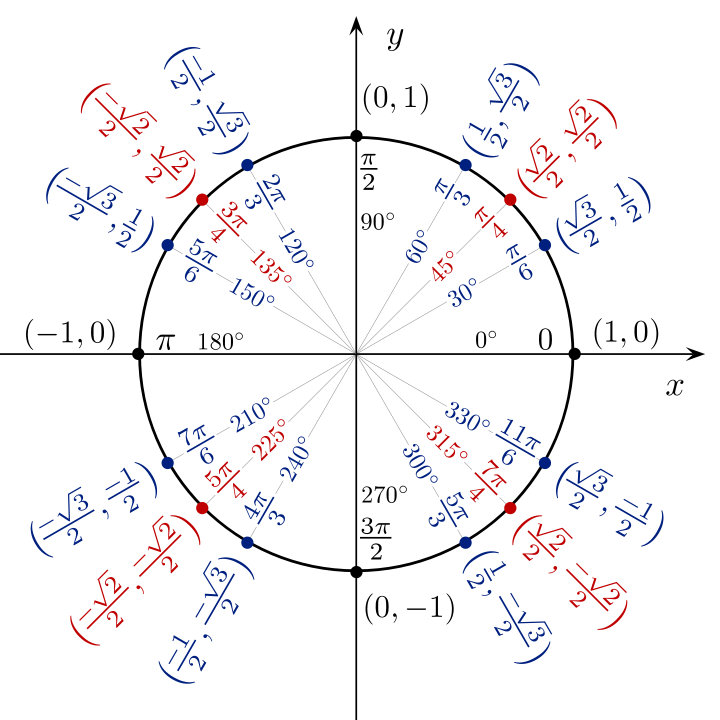
\includegraphics[width=0.5\textwidth]{Einheitskreis.png}
	\caption{Einheitskreis: (cos, sin)}
	\label{einheitskreis}
\end{figure}
Lese aus dem Einheitskreis (Abbildung \ref{einheitskreis}) ab:
\begin{enumerate}
	\item $\cos \frac{\pi}{4}$
	
	\ifshowsolution
		$\cos \frac{\pi}{4} = \frac{\sqrt{2}}{2}$
	\fi
	
	\item $\sin \frac{5\pi}{4}$
	
	\ifshowsolution
		$\sin \frac{5\pi}{4} = -\frac{\sqrt{2}}{2}$
	\fi
	
	\item $\acos{-\frac{\sqrt{3}}{2}}$
	
	\ifshowsolution
		$\acos{-\frac{\sqrt{3}}{2}} = \frac{5\pi}{6} \text{ bzw. } \frac{7\pi}{6}$
	\fi
	
	\item $\asin{-\frac{1}{2}}$
	
	\ifshowsolution
		$\asin{-\frac{1}{2}} = \frac{7\pi}{6} \text{ bzw. } \frac{11\pi}{6}$
	\fi
	
\end{enumerate}

\subsection{Komplexe Zahlen}
Gegeben seien folgende Zahlen aus $\mathbb{C}$. Bestimme den Real- und Imaginärteil, die komplex konjugierte so wie den Betrag: \\
Betrag: $\abs{x+yi} = \sqrt{x^2+y^2}$
\begin{enumerate}
	\item $2i - (2 + i) + (7 - 4i)$
	
	\ifshowsolution
		$2i - (2 + i) + (7 - 4i) = i-2 + (7-4i) = 5-3i$ \\
		Realteil: $5$ \\
		Imaginärteil: $-3$ \\
		Komplex Konjugierte: $5+3i$ \\
		Betrag: $\sqrt{5^2 + (-3)^2} = \sqrt{25+9} = \sqrt{34}$
	\fi
	
	\item $(1-i)^2$
	
	\ifshowsolution
		$(1-i)^2 = 1-2i+i^2 = 1-2i-1 = -2i$ \\
		Realteil: $0$ \\
		Imaginärteil: $-2$ \\
		Komplex Konjugierte: $2i$ \\
		Betrag: $\sqrt{(-2)^2} = \sqrt{4} = 2$
	\fi
	
	\item $\frac{3-i}{2+2i}$
	
	\ifshowsolution
		$\frac{3-i}{2+2i} = \frac{(3-i) \ \overline{(2+2i)}}{(2+2i) \ \overline{(2+2i)}} = \frac{(3-i)(2-2i)}{(2+2i)(2-2i)} = \frac{6-8i+2i^2}{4-4i^2} = \frac{6-8i-2}{4+4} = \frac{4-8i}{8} = \frac{1}{2}-i$ \\
		Realteil: $\frac{1}{2}$ \\
		Imaginärteil: $-1$ \\
		Komplex Konjugierte: $\frac{1}{2}+i$ \\
		Betrag: $\sqrt{\braces{\frac{1}{2}}^2+(-1)^2} = \sqrt{\frac{1}{4}+1} = \frac{\sqrt{5}}{2}$
	\fi
	
	\item $(2-i) + (3+i)(3-i)$
	
	\ifshowsolution
		$(2-i) + (3+i)(3-i) = (2-i) + (9-3i+3i-i^2) = 12-i$ \\
		Realteil: $12$ \\
		Imaginärteil: $-1$ \\
		Komplex Konjugierte: $12+i$ \\
		Betrag: $\sqrt{12^2 + (-1)^2} = \sqrt{145}$
	\fi
	
	\item $i^{\ 2015}$
	
	\ifshowsolution
		$i^{\ 2015} = i^{\ 503 \cdot 4 + 3} = i^{503 \cdot 4} \cdot i^3 = i^4 \cdot i^3 = 1 \cdot (-i) = 0-i$ \\
		Realteil: $0$ \\
		Imaginärteil: $-1$ \\
		Komplex Konjugierte: $0+i$ \\
		Betrag: $\sqrt{(-1)^2} = 1$
	\fi
\end{enumerate}

\subsubsection{Polarkoordinaten und Exponentialdarstellung Umwandlung}
Schreibe als Polarkoordinaten- und Exponentialdarstellung

Polarkoordinaten: $r(\cos \alpha + i \sin \alpha)$ mit $r=\sqrt{x^2+y^2}$ und $\acos{\frac{x}{r}} = \alpha = \asin{\frac{y}{r}}$

\begin{enumerate}
	\item $\sqrt{2}+\sqrt{2}i$
	
	\ifshowsolution
		$r = \sqrt{(\sqrt{2})^2 + (\sqrt{2})^2} = \sqrt{4} = 2$ \\
		$\cos \alpha = \frac{\sqrt{2}}{2} \quad \Rightarrow \quad \alpha = \acos{\frac{\sqrt{2}}{2}} \quad \Rightarrow \quad \alpha = \frac{\pi}{4} \lor \alpha = \frac{7\pi}{4}$ \\
		$\sin \alpha = \frac{\sqrt{2}}{2} \quad \Rightarrow \quad \alpha = \asin{\frac{\sqrt{2}}{2}} \quad \Rightarrow \quad \alpha = \frac{\pi}{4} \lor \alpha = \frac{3\pi}{4}$ \\
		Polarkoordinaten: $2 \braces{\cos \frac{\pi}{4} + i \sin \frac{\pi}{4}}$ \\
		Exponentialschreibweise: $2 e^{i \frac{\pi}{4}}$
	\fi
	
	\item $-4i$
	
	\ifshowsolution
		$r = \sqrt{(-4)^2} = 4$ \\
		$\cos \alpha = -\frac{0}{4} \quad \Rightarrow \quad \alpha = \acos{(0)} \quad \Rightarrow \quad \alpha = \frac{\pi}{2} \lor \alpha = \frac{3\pi}{2}$ \\
		$\sin \alpha = -\frac{4}{4} \quad \Rightarrow \quad \alpha = \asin{(-1)} \quad \Rightarrow \quad \alpha = \frac{3\pi}{2}$ \\
		Polarkoordinaten: $4 \braces{\cos \frac{3\pi}{2} + i \sin \frac{3\pi}{2}}$ \\
		Exponentialschreibweise: $4 e^{i \frac{3\pi}{2}}$
	\fi
	
	\item $6+2\sqrt{3}i$
	
	\ifshowsolution
		$r = \sqrt{6^2 + (2\sqrt{3})^2} = \sqrt{36 + 4 \cdot 3} = \sqrt{48} = 4 \sqrt{3}$ \\
		$\cos \alpha = \frac{6}{4\sqrt{3}} = \frac{\sqrt{3}}{2} \quad \Rightarrow \quad \alpha = \acos{\frac{\sqrt{3}}{2}} \quad \Rightarrow \quad \alpha = \frac{\pi}{6} \lor \alpha = \frac{11\pi}{6}$ \\
		$\sin \alpha = \frac{2\sqrt{3}}{4\sqrt{3}} = \frac{1}{2} \quad \Rightarrow \quad \alpha = \asin{\frac{1}{2}} \quad \Rightarrow \quad \alpha = \frac{\pi}{6} \lor \alpha = \frac{5\pi}{6}$ \\
		Polarkoordinaten: $4\sqrt{3} \braces{\cos \frac{\pi}{6} + i \sin \frac{\pi}{6} }$ \\
		Exponentialschreibweise: $4\sqrt{3} \cdot e^{i \frac{\pi}{6}}$
	\fi
\end{enumerate}

Schreibe als Summe von Real- und Imaginärteil (karthesische Darstellung: $x + yi$)

\begin{enumerate}
	\item $7 \braces{\cos \pi + i \sin \pi}$
	
	\ifshowsolution
		\begin{align*}
			7 \braces{\cos \pi + i \sin \pi} &= 7 \braces{-1 + i 0} \\
			&= -7
		\end{align*}
	\fi
	
	\item $\sqrt{3} \braces{\cos \frac{\pi}{3} + i \sin \frac{\pi}{3}}$
	
	\ifshowsolution
		\begin{align*}
			\sqrt{3} \braces{\cos \frac{\pi}{3} + i \sin \frac{\pi}{3}} &= \sqrt{3} \braces{\frac{1}{2} + i \frac{\sqrt{3}}{2}} \\
			&= \frac{\sqrt{3}}{2} + i \frac{3}{2}
		\end{align*}
	\fi
	
	\item $2 \cdot e^{i \frac{5 \pi}{3}}$
	
	\ifshowsolution
		\begin{align*}
			2 \cdot e^{i \frac{5 \pi}{3}} &= 2 \braces{\cos \frac{5\pi}{3} + i \sin \frac{5\pi}{3}} \\
			&= 2 \braces{\frac{1}{2} - i \frac{\sqrt{3}}{2}} \\
			&= 1 - i \sqrt{3}
		\end{align*}
	\fi
\end{enumerate}

\subsubsection{Rechnen in Polarkoordinaten}
Für 2 komplexe Zahlen $z_1$, $z_2$ mit Polarkoordinatendarstellung $z_i = r_i \braces{\cos \alpha_i + i \sin \alpha_i}$ gilt:

\begin{align*}
	z_1 \cdot z_2 &= r_1 r_2 \braces{ \cos \braces{\alpha_1 + \alpha_2} + i \sin \braces{\alpha_1 + \alpha_2}} \\
z_1 \div z_2 &= \frac{r_1}{r_2} \braces{\cos \braces{\alpha_1 - \alpha_2} + i \sin \braces{\alpha_1 - \alpha_2}} \\
z_1^n &= r_1^n \braces{\cos (n \alpha_1) + i \sin (n \alpha_1)} \\
	\sqrt[n]{z_1} &= w_k \text{ mit } w_k = \sqrt[n]{r_1} \braces{\cos \frac{\alpha_1 + 2k\pi}{n} + i \sin \frac{\alpha_1 + 2k\pi}{n}}, k = 0, \dots n-1
\end{align*}

Berechne in Polarkoordinaten:
\begin{enumerate}
	\item $3 \braces{\cos \frac{2\pi}{3} + i \sin \frac{2\pi}{3}} \cdot \sqrt{4} \braces{\cos \pi + i \sin \pi}$
	
	\ifshowsolution
		\begin{align*}
			3 \braces{\cos \frac{2\pi}{3} + i \sin \frac{2\pi}{3}} \cdot \sqrt{4} \braces{\cos \pi + i \sin \pi} &= 3 \sqrt{4} \braces{ \cos \braces{\frac{2\pi}{3}+\pi} + i \sin \braces{\frac{2\pi}{3} + \pi} } \\
			&= 6 \braces{ \cos \frac{5\pi}{3} + i \sin \frac{5\pi}{3} }
		\end{align*}
	\fi
		
	\item $4 \braces{ \cos \frac{7\pi}{6} + i \sin \frac{7\pi}{6} } \div 2 \braces{ \cos \pi + i \sin \pi }$
	
	\ifshowsolution
		\begin{align*}
			4 \braces{ \cos \frac{7\pi}{6} + i \sin \frac{7\pi}{6} } \div 2 \braces{ \cos \pi + i \sin \pi } &= \frac{4}{2} \braces{ \cos \braces{\frac{7\pi}{6} - \pi} + i \sin \braces{\frac{7\pi}{6} - \pi} } \\
			&= 2 \braces{\cos \frac{\pi}{6} + i \sin \frac{\pi}{6}}
		\end{align*}
	\fi
		
	\item $\braces{3+\sqrt{3}i}^4$
	
	\ifshowsolution
		$r = \sqrt{3^2 + \sqrt{3}^2} = \sqrt{12}, \quad \alpha = \acos{\frac{3}{\sqrt{12}}} = \acos {\frac{\sqrt{3}}{2}} = \frac{\pi}{6}$ \\
		\begin{align*}
			\braces{3+\sqrt{3}i}^4 &= \braces{ \sqrt{12} \braces{\cos \frac{\pi}{6} + i \sin \frac{\pi}{6}} }^4 \\
			&= \sqrt{12}^4 \braces{ \cos \frac{4\pi}{6} + i \sin \frac{4\pi}{6} } \\
			&= 12^2 \braces{ \cos \frac{2\pi}{3} + i \sin \frac{2\pi}{3} } \\
			&= 12^2 \braces{ - \frac{1}{2} + i \frac{\sqrt{3}}{2} } \\
			&= 72 + 72\sqrt{3}i
		\end{align*}
	\fi
		
	%TODO weitere Aufgabe zum Potenzieren und Wurzelziehen (mit besseren Zahlen)
	\item $p^4 + 16 = 0$
	
	\ifshowsolution
		% Dies lässt sich auch vereinfachen durch \sqrt[4]{-16} = \sqrt[4]{16 * i^2}
		\begin{align*}
			p^4 + 16 &= 0 \\
			p^4 &= -16 \\
			p &= \sqrt[4]{-16} \\
			\intertext{Wandle Radikanten in Polarkoordinaten um}
			r &= 16, \quad \alpha = \acos{\frac{-16}{16}} = \acos{-1} = \pi \\
			p &= \sqrt[4]{16 (\cos \pi + i \sin \pi)} \\
			\intertext{Nun können mit der Formel von oben die 4 Nullstellen bestimmt werden}
			w_0 &= \sqrt[4]{16} \braces{\cos \frac{\pi + 0\pi}{4} + i \sin \frac{\pi + 0\pi}{4} } = 2 \braces{ \frac{\sqrt{2}}{2} + i \frac{\sqrt{2}}{2} } = \sqrt{2} + i \sqrt{2} \\
			w_1 &= \sqrt[4]{16} \braces{\cos \frac{\pi + 2\pi}{4} + i \sin \frac{\pi + 2\pi}{4} } = 2 \braces{ -\frac{\sqrt{2}}{2} + i \frac{\sqrt{2}}{2} } = -\sqrt{2} + i \sqrt{2} \\
			\intertext{Prinzipiell kann man nun die anderen beiden Lösungen sofort ablesen, da zu jeder Lösung $x + yi$ auch ihre konjugierte $x - yi$ eine Lösung ist.}
			w_2 &= \sqrt[4]{16} \braces{\cos \frac{\pi + 4\pi}{4} + i \sin \frac{\pi + 4\pi}{4} } = 2 \braces{ -\frac{\sqrt{2}}{2} - i \frac{\sqrt{2}}{2} } = -\sqrt{2} - i \sqrt{2} \\
			w_3 &= \sqrt[4]{16} \braces{\cos \frac{\pi + 6\pi}{4} + i \sin \frac{\pi + 6\pi}{4} } = 2 \braces{ \frac{\sqrt{2}}{2} - i \frac{\sqrt{2}}{2} } = \sqrt{2} - i \sqrt{2} \\
		\end{align*}
	\fi
\end{enumerate}

\subsection{Folgen}
\subsubsection{DGL}
\begin{description}
	\item[Folgen 1. Ordnung] $a_{n+1} = q \cdot a_n + d$
		\begin{align*}
			a_n = \begin{cases}
				a_0 \cdot q^n + d \cdot \frac{1-q^n}{1-q}, &\text{ falls } q \in \mathbb{R} \setminus \{1\} \\
				a_0 + d \cdot n &\text{ falls } q=1
					\end{cases}
		\end{align*}
	\item[Folgen 2. Ordnung] $a_{n+1} = b a_n + c a_{n-1}$ \vspace{0.3cm} \\
		Für das charakteristisches Polynom $q^2 = bq+c$ mit Nullstellen $q_1, q_2$ gibt die folgende Tablle in Abhängigkeit davon, ob bei der PQ-Formel der Teil unter der Wurzel positiv, $0$ oder negativ ist, die explizite Form an.
		
		\begin{tabular}{|c|l|}
			\hline
			Diskriminante & Explizite Darstellung \\ \hline
			$>0$ & $a_n = C_1 q_1^n + C_2 q_2^n$ \\
			$=0$ & $a_n = C_1 q_1^n + C_2 n \cdot q_2^n$ \\
			$<0$ & $a_n = C_1 r^n \cos(n\alpha) + C_2 r^n \sin(n\alpha)$ \\ \hline
		\end{tabular}
\end{description}

Finde die explizite Darstellung von $a_n$. Gib auch den Grenzwert $\lim_{n \rightarrow \infty} a_n$ an.
\begin{enumerate}
	\item $a_{n+1} = 3 a_n + 6$ mit $n \in \mathbb{N}_0,\ a_0 = 4$ \label{DGLAufgabe1}
	
	\ifshowsolution
		$q=3 (\neq 1), \quad d=6$
		\begin{align*}
			a_n &= 4 \cdot 3^n + 6 \frac{1-3^n}{1-3} \\
			a_n &= 4 \cdot 3^n - 3 (1-3^n) \\
			a_n &= 4 \cdot 3^n - 3 + 3 \cdot 3^n \\
			a_n &= 7 \cdot 3^n - 3 \tag{Explizite Darstellung}
		\end{align*}
		$\lim_{n \rightarrow \infty} 7 \cdot 3^n - 3 = +\infty$
	\fi
		
	\item $a_{n+1} = 2 a_n +2$ mit $n \in \mathbb{N}_0,\ a_1 = 4$
	
	\ifshowsolution
		$q=2, \quad d=2 \quad a_0 = ?$ \\
		Wir haben $a_1$ gegeben, brauchen aber $a_0$. Setze $n$ so ein, dass in der Formel sowohl $a_1$ als auch $a_0$ vorkommen. Dann kann nach $a_0$ umgestellt werden.
		\begin{align*}
			a_1 &= 2 a_0 +2 \\
			4 &= 2 a_0 +2 \\
			1 &= a_0
		\end{align*}
		Nun weiter wie bei \ref{DGLAufgabe1}:
		\begin{align*}
			a_n &= 1 \cdot 2^n + 2 \cdot \frac{1-2^n}{1-2} \\
			a_n &= 2^n - 2 \cdot \braces{1-2^n} \\
			a_n &= 2^n - 2 + 2 \cdot 2^n \\
			a_n &= 3 \cdot 2^n - 2
		\end{align*}
		$\lim_{n \rightarrow \infty} 3 \cdot 2^n - 2 = +\infty$
	\fi
		
	\item $a_{n+2} = 5 a_{n+1} - 3$ mit $n \in \mathbb{N}_0,\ a_0 = 1$
	
	\ifshowsolution
		\begin{align*}
			a_{n+1} &= 5 a_{n} - 3 \tag{Index-Shift} \\
			q &= 5, \quad d = -3 \\
			a_n &= 1 \cdot 5^n -3 \cdot \frac{1-5^n}{1-5} \\
			a_n &= 5^n + \frac{3}{4} \cdot (1-5^n) \\
			a_n &= \frac{5^n+3}{4}
		\end{align*}
		$\lim_{n \rightarrow \infty} \frac{5^n+3}{4} = +\infty$
	\fi
		
	\item $a_{n+1} = -6 a_{n} - 5 a_{n-1}$ mit $a_0=2, a_1=4$
	
	\ifshowsolution
		$b=-6, c=-5$ \\
		Charakteristische Gleichung: $q^2 = -6q -5 \ \Leftrightarrow \ 0 = q^2 + 6q + 5$ \\
		Mit der PQ-Formel folgt $q_1=-1, q_2=-5$ \\
		Die explizite Form lautet also $a_n = C_1 (-1)^n + C_2 (-5)^n$ \\ \\
		$C_1$, $C_2$ müssen nun noch aus den Anfangsbedingungen bestimmt werden: \\
		$a_0 = 2 = C_1 (-1)^0 + C_2 (-5)^0 \Leftrightarrow C_1 + C_2 = 2$ \\
		$a_1 = 4 = C_1 (-1)^1 + C_2 (-5)^1 \Leftrightarrow -C_1 -5C_2 = 4$ \\
		LGS Lösen: $C_1=\frac{7}{2}, C_2=-\frac{3}{2}$ \\
		$a_n = \frac{7}{2} (-1)^n - \frac{3}{2} (-5)^n$ \\
		$\lim_{n \rightarrow \infty} \frac{7}{2} (-1)^n - \frac{3}{2} (-5)^n = \tilde{\infty}$ (Alternierend, divergent)
	\fi
		
	\item $a_{n+1} = 3 a_n - 4 a_{n-1}$ mit $a_0=3, a_1=4$
	
	\ifshowsolution
		$b=3, c=4$ \\
		Charakteristische Gleichung: $q^2 = 3q - 4 \Leftrightarrow 0 = q^2 - 3q + 4$ \\
		$q_1=\frac{3}{2} + i \frac{\sqrt{7}}{2}, q_2=\frac{3}{2} - i \frac{\sqrt{7}}{2}$ \\
		In Polarkoordinaten: $r^2 = \frac{3}{2}^2 + \frac{\sqrt{7}}{2}^2, \alpha = \acos{\frac{\frac{3}{2}}{2}} = \acos{\frac{3}{4}} \approx 0.72$ \\
		$a_n = C_1 \cdot 2^n \cos(n\cdot 0.72) + C_2 \cdot 2^n \sin(n \cdot 0.72)$ \\ \\
		$C_1$, $C_2$ aus Anfangsbedingungen: \\
		$a_0 = 3 = C_1 \cos(0) + C_2 \sin(0) \Leftrightarrow 3 = C_1$ \\
		$a_1 = 4 = C_1 \cdot 2 \cos(\cdot 0.72) + C_2 \cdot 2 \sin(\cdot 0.72) \Leftrightarrow 4 = 6 \cdot \frac{3}{4} + C_2 \cdot 2 \cdot 0.66 \Leftrightarrow C_2 \approx -\frac{25}{66}$ \\
		Die Lösung lautet also: $a_n = 3 \cdot 2^n \cos(n\cdot 0.72) -\frac{25}{66} \cdot 2^n \sin(n \cdot 0.72)$ \\
		$\lim_{n \rightarrow \infty} 3 \cdot 2^n \cos(n\cdot 0.72) -\frac{25}{66} \cdot 2^n \sin(n \cdot 0.72) = \tilde{\infty}$ (Alternierend, divergent)
	\fi
\end{enumerate}

\subsection{Reihen}
\subsubsection{Konvergenz und Divergenz}
Konvergieren die folgenden Reihen?
\begin{enumerate}
	\item $\sum_{k=0}^\infty \frac{(2k+2)(3k-2)}{(2k-2)^2}$
	
	\ifshowsolution
		\begin{align*}
			a_k &= \frac{(2k+2)(3k-2)}{(2k-2)^2} \\
			&= \frac{6k^2+2k-4}{4k^4-8k+4}
		\end{align*}
		$\lim_{k->\infty} a_k = \frac{3}{2} \neq 0$, die Reihe divergiert.
	\fi
		
	\item $\sum_{k=0}^\infty \frac{(k-1)^2}{\sqrt{3^k}}$
	
	\ifshowsolution
		\begin{align*}
			\lambda &= \lim_{k->\infty} \abs{ \frac{\frac{k^2}{\sqrt{3^{k+1}}}}{\frac{(k-1)^2}{\sqrt{3^k}}} } \tag{Quotientenkriterium} \\
			&= \lim_{k->\infty} \abs{ \frac{\frac{\sqrt{3^k} k^2}{\sqrt{3^{k+1}}}}{(k-1)^2} } \\
			&= \lim_{k->\infty} \abs{ \frac{k^2 \frac{\sqrt{3^k}}{\sqrt{3^{k+1}}}}{(k-1)^2} } \\
			&= \lim_{k->\infty} \abs{ \frac{k^2 \sqrt{\frac{3^k}{3^{k+1}}}}{(k-1)^2} } \\
			&= \lim_{k->\infty} \abs{ \frac{k^2 \sqrt{\frac{1}{3}}}{k^2-2k+1} } \\
			\intertext{Der Grenzwert des Bruches ist der Quotient der Koeffizienten am größten Term, also}
			\lambda &= \sqrt{\frac{1}{3}}
		\end{align*}
		Lambda ist $<1$, laut Quotientenkriterium ist die Reihe damit (absolut) konvergent.
	\fi
		
	\item $\sum_{k=2}^\infty \frac{\sqrt{2k-1}}{k^2-k+\frac{1}{4}}$
	
	\ifshowsolution
		\begin{align*}
			\shortintertext{Die Konvergenz der Reihe $\sum_{k=1}^\infty \frac{1}{k^2}$ ist aus der Vorlesung bekannt}
			\frac{\sqrt{2k-1}}{k^2-k+\frac{1}{4}} &\leq \frac{1}{k^2} \\
			\frac{\sqrt{2} \cdot \sqrt{k+\frac{1}{2}}}{(k-\frac{1}{2})^2} &\leq \frac{1}{k^2} \\
			\frac{2 \cdot (k+\frac{1}{2})}{(k-\frac{1}{2})^4} &\leq \frac{1}{k^2} \\
			\frac{2}{(k-\frac{1}{2})^3} &\leq \frac{1}{k^2}
		\end{align*}
		Nach dem Majorantenkriterium ist diese Reihe also (absolut) konvergent.
	\fi
\end{enumerate}

\subsubsection{Grenzwerte}
Konvergieren die folgenden Reihen? Wenn ja, berechne auch den Grenzwert. Der folgende Satz für die geometrische Reihe könnte nützlich werden:

Bei $\abs{q}<1$ gilt die für geometrische Reihe $\sum_{k=0}^\infty q^k = \frac{1}{1-q}$.
\begin{enumerate}
	\item $\sum_{k=4}^\infty \frac{1}{k^2-5k+6}$
	
	\ifshowsolution
		\begin{align*}
			\intertext{Zunächst formen wir die Reihenglieder $a_k$ um}
			a_k &= \frac{1}{k^2-5k+6} \\
			&= \frac{1}{(k-2)(k-3)} \\
			&= \frac{(k-2)-(k-3)}{(k-2)(k-3)} \\
			&= \frac{\cancel{(k-2)}}{\cancel{(k-2)}(k-3)} - \frac{\cancel{(k-3)}}{(k-2)\cancel{(k-3)}} \\
			&= \frac{1}{k-3} - \frac{1}{k-2}		
			\intertext{Dann betrachten wir die Partialsumme $S_n = \sum_{k=4}^n a_k$ (es gilt $\lim_{n \rightarrow \infty} S_n = \sum_{k=0}^\infty a_k$). Das manuelle aufaddieren der Elemente von $S_n$ entlarvt die Reihe als 'Teleskopsumme', bei der sich so gut wie alle Terme rauskürzen lassen:}
			\sum_{k=4}^n a_k = \frac{1}{1} &- \cancel{\frac{1}{2}} \tag{$k=4$} \\
			+ \cancel{\frac{1}{2}} &- \cancel{\frac{1}{3}} \tag{$k=5$} \\
			& \vdots \\
			+ \cancel{\frac{1}{n-4}} &- \cancel{\frac{1}{n-3}} \tag{$k=n-1$} \\
			+ \cancel{\frac{1}{n-3}} &- \frac{1}{n-2} \tag{$k=n$}
		\end{align*}
		Es folgt nun:
		\begin{align*}
			\sum_{k=4}^\infty a_k &= \lim_{n \rightarrow \infty} S_n \\
			&= \lim_{n \rightarrow \infty} 1 - \frac{1}{n-2} \\
			&= 1
		\end{align*}
		Damit konvergierte die Reihe also gegen 1.
	\fi
		
	\item $\sum_{k=0}^\infty \frac{2}{k^2+6k+8}$
	
	\ifshowsolution
		\begin{align*}
			\intertext{Zunächst formen wir die Reihenglieder $a_k$ um}
			a_k &= \frac{2}{k^2+6k+8} \\
			&= \frac{2}{(k+2)(k+4)} \\
			&= \frac{(k+4)-(k+2)}{(k+2)(k+4)} \\
			&= \frac{\cancel{(k+4)}}{(k+2)\cancel{(k+4)}} - \frac{\cancel{(k+2)}}{\cancel{(k+2)}(k+4)} \\
			&= \frac{1}{k+2} - \frac{1}{k+4}
			\intertext{Dann betrachten wir die Partialsumme $S_n = \sum_{k=4}^n a_k$ (es gilt $\lim_{n \rightarrow \infty} S_n = \sum_{k=0}^\infty a_k$). Das manuelle aufaddieren der Elemente von $S_n$ entlarvt die Reihe als 'Teleskopsumme', bei der sich so gut wie alle Terme rauskürzen lassen:}
			\frac{1}{2} &- \cancel{\frac{1}{4}} \tag{$k=0$} \\
			\frac{1}{3} &- \cancel{\frac{1}{5}} \tag{$k=1$} \\
			\cancel{\frac{1}{4}} &- \cancel{\frac{1}{6}} \tag{$k=2$} \\
			\cancel{\frac{1}{5}} &- \cancel{\frac{1}{7}} \tag{$k=3$} \\
			& \vdots \\
			\cancel{\frac{1}{n}} &- \cancel{\frac{1}{n+2}} \tag{$k=n-2$} \\
			\cancel{\frac{1}{n+1}} &- \frac{1}{n+3} \tag{$k=n-1$} \\
			\cancel{\frac{1}{n+2}} &- \frac{1}{n+4} \tag{$k=n$} \\
		\end{align*}
		Es gilt also:
		\begin{align*}
			\sum_{k=0}^\infty a_k &= \lim_{n \rightarrow \infty} S_n \\
			&= \lim_{n \rightarrow \infty} \frac{1}{2} + \frac{1}{3} - \frac{1}{n+3} - \frac{1}{n+4} \\
			&= \frac{5}{6}
		\end{align*}
		Damit ist $\sum_{k=0}^\infty \frac{2}{k^2+6k+8} = \frac{5}{6}$
	\fi
		
	\item $\sum_{k=0}^\infty \frac{(-1)^k \cdot 2^{k-1} - 5 \cdot 6^k}{4^{2k+1}}$
	
	\ifshowsolution
		\begin{align*}
			\intertext{Zunächst formen wir die Reihenglieder um (unter Verwendung vieler Potenzgesetze)}
			a_k &= \frac{(-1)^k \cdot 2^{k-1} - 5 \cdot 6^k}{4^{2k+1}} \\
			&= \frac{(-1)^k \cdot \frac{2^k}{2} - 5 \cdot 6^k}{4 \cdot 4^{2k}} \\
			&= \frac{\frac{-2^k}{2} - 5 \cdot 6^k}{4 \cdot 16^k} \\
			&= \frac{\frac{-2^k}{2}}{4 \cdot 16^k} - \frac{5 \cdot 6^k}{4 \cdot 16^k} \\
			&= \frac{1}{8} \cdot \frac{-2^k}{16^k} - \frac{5}{4} \cdot \frac{6^k}{16^k} \\
			&= \frac{1}{8} \cdot \braces{-\frac{2}{16}}^k - \frac{5}{4} \cdot \braces{\frac{6}{16}}^k \\
			&= \frac{1}{8} \cdot \braces{-\frac{1}{8}}^k - \frac{5}{4} \cdot \braces{\frac{3}{8}}^k
			\intertext{Wenden wir uns nun wieder der gesammten Reihe zu}
			\sum_{k=0}^\infty a_k &= \sum_{k=0}^\infty \braces{\frac{1}{8} \cdot \braces{-\frac{1}{8}}^k - \frac{5}{4} \cdot \braces{\frac{3}{8}}^k} \\
			&= \sum_{k=0}^\infty \frac{1}{8} \cdot \braces{-\frac{1}{8}}^k - \sum_{k=0}^\infty \frac{5}{8} \cdot \braces{\frac{3}{8}}^k \\
			&= \frac{1}{8} \underbrace{\sum_{k=0}^\infty \braces{-\frac{1}{8}}^k}_{\text{geom. Reihe}} - \frac{5}{8} \underbrace{\sum_{k=0}^\infty \braces{\frac{3}{8}}^k}_{\text{geom. Reihe}} \\
			&= \frac{1}{8} \cdot \frac{1}{1-\braces{-\frac{1}{8}}} - \frac{5}{4} \cdot \frac{1}{1-\frac{3}{8}} \\
			\intertext{Dies lässt sich vereinfachen zum Grenzwert der Reihe}
			&= -\frac{17}{9}
		\end{align*}
	\fi
\end{enumerate}

\subsection{Logarithmen}
Wichtige Rechenregeln für Logarithmen sind:
\begin{align*}
	\log a + \log b &= \log ab \\
	\log a - \log b &= \log \frac{a}{b} \\
	c \cdot \log a &= \log \braces{a^c} \\
	\log_a x &= \frac{\log_b x}{\log_b a}
\end{align*}

Löse die folgenden Gleichungen:
\begin{enumerate}
	\item $\frac{1}{2} \log x + \log \sqrt{x-1} = \log \sqrt{2}$
	
	\ifshowsolution
		\begin{align*}
			\frac{1}{2} \log x + \log \sqrt{x-1} &= \log \sqrt{2} \\
			\frac{1}{2} \log x + \log (x-1)^\frac{1}{2} &= \log 2^\frac{1}{2} \\
			\frac{1}{2} \log x + \frac{1}{2} \log (x-1) &= \frac{1}{2} \log 2 \\
			\intertext{Durch Multiplizieren mit 2 auf beiden Seiten ergibt sich}
			\log x + \log (x-1) &= \log 2 \\
			\log x + \log (x-1) - \log 2 &= 0 \\
			\intertext{Nach den Rechenregeln von oben können wir das schreiben als}
			\log \frac{x (x-1)}{2} &= 0 \\
			\intertext{Nun wenden wir auf beiden Seiten die $e$-Funktion an, so dass der Logarithmus verschwindet. Anm: $e^0 = 1$}
			\frac{x (x-1)}{2} &= 1 \\
			x^2 - x - 2 &= 0 \\
			\Rightarrow \quad x_1 = 2, \quad x_2 &= -1
		\end{align*}
		Die Logarithmusregeln die wir genutzt haben gelten nur für logartihmen mit nicht-negativem Argument, daher ist eine Probe nötig. $x_2 = -1$ liegt nicht im Definitionsbereich des Logarithmus und ist daher keine Lösung. Für $x_1 = 2$ gilt: \\
		\begin{align*}
			\frac{1}{2} \log 2 + \log \sqrt{1} = \log \sqrt{2} \\
			\log \sqrt{2} = \log \sqrt{2}
		\end{align*}
	\fi
	
	\item $\log_{10} \braces{15 \cdot 50^x + 2 \cdot 2^x} = \log_{10} 15 + x$
	
	\ifshowsolution
		\begin{align*}
			\log_{10} \braces{15 \cdot 50^x + 2 \cdot 2^x} &= \log_{10} 15 + x \\
			\log_{10} \braces{15 \cdot 50^x + 2 \cdot 2^x} &= \log_{10} 15 + \log_{10} 10^x \\
			\log_{10} \braces{15 \cdot 50^x + 2 \cdot 2^x} &= \log_{10} (15 \cdot 10^x) \\
			15 \cdot 50^x + 2 \cdot 2^x &= 15 \cdot 10^x \\
			15 \cdot 50^x + 2 \cdot 2^x - 15 \cdot 10^x &= 0 \\
			\intertext{Wegen $(ab)^x = a^x b^x$ können wir nun aus jedem Exponentialterm $2^x$ rausziehen.}
			15 \cdot 2^x \cdot (25)^x + 2 \cdot 2^x - 15 \cdot 2^x \cdot 5^x &= 0 \\
			\underbrace{2^x}_{\neq 0} \braces{15 \cdot (25)^x + 2 - 15 \cdot 5^x} &= 0 \\
			15 \cdot (5^2)^x - 15 \cdot 5^x + 2 &= 0 \\
			15 \cdot (5^x)^2 - 15 \cdot 5^x + 2 &= 0
			\shortintertext{Substitution: Sei $y = 5^x$}
			15 \cdot y^2 - 15 \cdot y + 2 &= 0 \\
			y^2 - y + \frac{2}{15} &= 0
			\shortintertext{Aus der PQ-Formel ergibt sich: $y_1 \approx 0.8416,\ y_2 \approx 0.1584$. Nun durch Rücksubstitution nach x auflösen:}
			5^x = 0.8416 \Leftrightarrow \log_5 0.8416 = x \Leftrightarrow x &\approx -0.107175302 \\
			5^x = 0.1584 \Leftrightarrow \log_5 0.1584 = x \Leftrightarrow x &\approx -1.14475433
		\end{align*}
	\fi
\end{enumerate}

\subsection{Analysis}
\subsubsection{Partialbruchzerlegung}
Berechne mittels PBZ:
\begin{enumerate}
	\item $\displaystyle \int_4^6 \frac{3x}{x^2 - 2x - 3} dx$ % Faktorisierung (x+1)(x-3)
	
	\ifshowsolution
		\begin{align*}
			\int_4^6 \frac{3x}{x^2 - 2x - 3} dx &= \int_4^6 \frac{3x}{(x-3)(x+1)} dx \\
			\intertext{Zunächst machen wir folgenden Ansatz}
			\frac{3x}{(x-3)(x+1)} &= \frac{A}{x-3} + \frac{B}{x+1} \label{eq:pbz-ansatz} \\
			&= \frac{A (x+1)}{(x-3)(x+1)} + \frac{B (x-3)}{(x-3)(x+1)} \\
			&= \frac{A (x+1) + B (x-3)}{(x-3)(x+1)} \\
			\intertext{Das gleichsetzen der Zähler ergibt}
			3x &= A (x+1) + B (x-3) \\
			\intertext{Der Koeffizientenvergleich führt dann zu einem Gleichungssystem}
			\underline{3x} + \uwave{0} &= \underline{Ax + Bx} + \uwave{A -3B} \\
			\rightarrow \begin{cases}
				3 = A + B \\
				0 = A - 3B
			\end{cases}
			\quad &\Leftrightarrow \quad A = \frac{9}{4}, \quad B = \frac{3}{4} \\
			\intertext{Die so ausgerechneten $A$ und $B$ setzen wir nun wieder in den Ansatz ein}
			\frac{3x}{(x-3)(x+1)} &= \frac{\frac{9}{4}}{x-3} + \frac{\frac{3}{4}}{x+1} \\
			\intertext{Nun lässt sich das Integral leicht lösen}
			\int_4^6 \frac{3x}{(x-3)(x+1)} dx &= \int_4^6 \frac{\frac{9}{4}}{x-3} + \frac{\frac{3}{4}}{x+1} dx \\
			&= \int_4^6 \frac{\frac{9}{4}}{x-3} dx + \int_4^6 \frac{\frac{3}{4}}{x+1} dx \\
			\intertext{Mit $\int \frac{1}{a} = \ln{a}$ folgt}
			&= \frac{9}{4} \int_4^6 \frac{1}{x-3} dx + \frac{3}{4} \int_4^6 \frac{1}{x+1} dx \\
			&= \frac{9}{4} \left. \ln(x-3) \right|_4^6 + \frac{3}{4} \left. \ln(x+1) \right|_4^6 \\
			&\approx 2.7242
		\end{align*}
	\fi
	
	\item $\displaystyle \int_2^3 \frac{x-1}{x^3 + 4x^2 + 5x + 2} dx$ % Faktorisierung (x+1)^2(x+2)
	
	\ifshowsolution
		\begin{align*}
			\intertext{Polynom dritten Grades: eine Nullstelle raten, dann per Polynomdivision faktorisieren}
			\int_2^3 \frac{x-1}{x^3 + 4x^2 + 5x + 2} dx &= \int_2^3 \frac{x-1}{(x+1)^2 (x+2)} dx \\
			\intertext{Bei einem Polynom dritten Grades sieht der Ansatz folgendermaßen aus}
			\frac{x-1}{(x+1)^2 (x+2)} &= \frac{A}{x+1} + \frac{B}{(x+1)^2} + \frac{C}{x+2} \\
			&= \frac{A(x+1)(x+2) + B(x+2) + C(x+1)^2}{(x+1)^2 (x+2)} \\
			\intertext{Wir setzen die Zähler gleich und erhalten durch Koeffizientenvergleich ein Gleichungssystem}
			x-1 &= A(x+1)(x+2) + B(x+2) + C(x+1)^2 \\
			\underline{\underline{0x^2}} + \underline{x} \ \uwave{- 1} &=
			\underline{\underline{Ax^2}} + \underline{3Ax} + \uwave{2A} + \underline{Bx} + \uwave{2B} + \underline{\underline{Cx^2}} + \underline{2Cx} + \uwave{C} \\
			\rightarrow \begin{cases}
				0 = A + C \\
				1 = 3A + B + 2C \\
				-1 = 2A + 2B + C
			\end{cases}
			&\rightarrow \begin{cases}
				C = -A \\
				1 = A + B \\
				-2 = B
			\end{cases} \\
			&\Rightarrow A=3, B=-2, C=-3 \\
			\intertext{Einsetzen der Werte für $A$, $B$ und $C$ in den Ansatz ergibt}
			\frac{x-1}{(x+1)^2 (x+2)} &= \frac{3}{x+1} - \frac{2}{(x+1)^2} - \frac{3}{x+2} \\
			\intertext{Das Integral kann mit dieser Form gelöst werden.}
			\int_2^3 \frac{x-1}{x^3 + 4x^2 + 5x + 2} dx &= \int_2^3 \frac{3}{x+1} - \frac{2}{(x+1)^2} - \frac{3}{x+2} dx \\
			&= \int_2^3 \frac{3}{x+1} dx - \int_2^3 \frac{2}{(x+1)^2} dx - \int_2^3 \frac{3}{x+2} dx \\
			&= 3 \left. \ln(x+1) \right|_2^3 + \left. \frac{2}{x+2} \right|_2^3 - 3 \left. \ln(x+2) \right|_2^3 \\
			&\approx 0.0269
		\end{align*}
	\fi
\end{enumerate}

\subsubsection{Substitution}
\begin{align*}
	\int_a^b \mathrm{f}( \ \underbrace{\mathrm{g}(x)}_t \ ) g'(x) \intend{x} = \int_{\mathrm{g}(a)}^{\mathrm{g(b)}} \mathrm{f}(t) \intend{t}
\end{align*}

Berechne mittels Substitution:
\begin{enumerate}
	\item $\int_{-\pi}^\pi \sin{x} \cdot \cos{x} \intend{x}$
	
	\ifshowsolution
		\begin{align*}
			\shortintertext{Substituiere: $\sin{x} = t$}
			\shortintertext{$\frac{dt}{dx} = \cos{x} \Leftrightarrow \intend{x} = \frac{\intend{t}}{\cos{x}}$}
			\int_{-\pi}^\pi \sin{x} \cdot \cos{x} \intend{x} &= \int_{\sin{-\pi}}^{\sin{\pi}} t\ \cancel{\cos{x}}\ \frac{\intend{t}}{\cancel{\cos{x}}} \\
			&= \int_{\sin{-\pi}}^{\sin{\pi}} t \intend{t} \\
			&= \brackets{\frac{1}{2} t^2}_{\sin{-\pi}}^{\sin{\pi}} \\
			&= \frac{1}{2} \brackets{t^2}_0^0 \\
			&= 0
		\end{align*}
	\fi
	
	\item $\int_1^e \frac{\sqrt{\ln(x)}}{x} \intend{x}$
	
	\ifshowsolution
		\begin{align*}
			\shortintertext{Substituiere: $\ln(x) = t$}
			\shortintertext{$\frac{\intend{t}}{\intend{x}} = \frac{1}{x} \Leftrightarrow \intend{x} = x \intend{t}$}
			\int_1^e \frac{\sqrt{\ln(x)}}{x} dx &= \int_{\ln(1)}^{\ln(e)} \sqrt{z} \intend{t} \\
			&= \int_0^1 \sqrt{z} \intend{t} \\
			&= \brackets{ \frac{2}{3} z^{\frac{3}{2}} }_0^1 \\
			&= \frac{2}{3}
			\shortintertext{Oder: Rücksubstitution nach Integration}
			\brackets{ \frac{2}{3} z^{\frac{3}{2}} }_0^1 &= \brackets{ \frac{2}{3} \ln(x)^{\frac{3}{2}} }_1^e \\
			&= \frac{2}{3}
		\end{align*}
	\fi
	
	\item $\int_\frac{\pi}{2}^\pi e^{3 \cos x} \cdot \sin x \intend{x}$
	
	\ifshowsolution
		\begin{align*}
			\shortintertext{Substituiere: $3 \cos x = t$}
			\shortintertext{$\frac{\intend{t}}{\intend{x}} = -3 \sin x \Leftrightarrow \intend{x} = \frac{\intend{t}}{-3 \sin x}$}
			\int_\frac{\pi}{2}^\pi e^{3 \cos x} \cdot \sin x \intend{x} &= \int_{t\braces{\frac{\pi}{2}}}^{t\braces{\pi}} e^t \cdot \cancel{\sin x} \ \frac{\intend{t}}{-3 \ \cancel{\sin x}} \\
			&= \int_{t\braces{\frac{\pi}{2}}}^{t\braces{\pi}} e^t \frac{1}{-3} \intend{t} \\
			&= -\frac{1}{3} \int_{t\braces{\frac{\pi}{2}}}^{t\braces{\pi}} e^t\intend{t} \\
			&= -\frac{1}{3} \brackets{e^t}_{t\braces{\frac{\pi}{2}}}^{t\braces{\pi)}} \\
			&= -\frac{1}{3} \brackets{e^t}_{3 \cos(\frac{\pi}{2})}^{3 \cos(\pi)} \\
			&= -\frac{1}{3} \brackets{e^t}_0^{-3} \\
			&= -\frac{1}{3} \braces{e^{-3} - 1}
			\shortintertext{Oder: Rücksubstitution nach Integration}
			-\frac{1}{3} \left[ e^t \right]_{t(\frac{\pi}{2})}^{t(\pi)} &= -\frac{1}{3} \left[ e^{3 \cos x} \right]_{\frac{\pi}{2}}^\pi \\
			&= -\frac{1}{3} \braces{e^{3 \cos \pi} - e^{3 \cos \frac{\pi}{2}}} \\
			&= -\frac{1}{3} \braces{e^{-3} - 1}
		\end{align*}
	\fi
\end{enumerate}

\subsubsection{Partielle Integration}
\begin{align*}
	\int \mathrm{f}(x) \ \mathrm{g}'(x) \intend{x} = \brackets{\mathrm{f}(x) \ \mathrm{g}(x)} - \int \mathrm{f}'(x) \ \mathrm{g}(x) \intend{x}
\end{align*}

Berechne mittels partieller Integration:
\begin{enumerate}
	\item $\int_0^1 3x^2 e^x \intend{x}$
	
	\ifshowsolution
		\begin{align*}
			\int_0^1 \underbrace{3x^2}_\mathrm{f} \underbrace{e^x}_\mathrm{g'} \intend{x} &= \brackets{3x^2 e^x}_0^1 - \int_0^1 \underbrace{6x}_\mathrm{f} \ \underbrace{e^x}_\mathrm{g'} \intend{x} \\
			&= \brackets{3x^2 e^x}_0^1 - \braces{ \brackets{6x \ e^x}_0^1 - \int_0^1 6 e^x \intend{x} } \\
			&= \brackets{3x^2 e^x}_0^1 - \brackets{6x \ e^x}_0^1 + 6 \int_0^1 e^x \intend{x} \\
			&= \brackets{3x^2 e^x}_0^1 - \brackets{6x \ e^x}_0^1 + 6 \brackets{e^x}_0^1 \\
			&= 3e - 6
		\end{align*}
	\fi
\end{enumerate}

%%%%%%%%%%%%%%%%%%%%%%%%%%%%%%%%%%%%%%%%%%%%%%%%%%%%%%%%%%%%%%%%%%%%%%%%%%%%%%%%
%                                Statistik                                     %
%%%%%%%%%%%%%%%%%%%%%%%%%%%%%%%%%%%%%%%%%%%%%%%%%%%%%%%%%%%%%%%%%%%%%%%%%%%%%%%%
\newpage
\section{Statistik}
\subsection{Klassische Wahrscheinlichkeitsrechnung}
\subsubsection{Würfel}
Ein fairer Würfel wird geworfen. Wie groß ist die Wahrscheinlichkeit, dass \dots \\

\begin{enumerate}
	\item eine 3 geworfen wird?
	
	\ifshowsolution
		Ereignisraum $\Omega = \{1,2,3,4,5,6\}, \quad \abs{\Omega} = 6$ \\
		$\abs{\{3\}} = 1 \rightarrow P(3) = \frac{1}{6}$
	\fi
	
	\item eine 3 oder eine 4 geworfen wird?
	
	\ifshowsolution
		Ereignisraum $\Omega = \{1,2,3,4,5,6\}, \quad \abs{\Omega} = 6$ \\
		$\abs{\{3, 4\}} = 2 \rightarrow P(3 \cup 4) = \frac{2}{6}$
	\fi
	
	\item eine Primzahl $> 3$ geworfen wird?
	
	\ifshowsolution
		Ereignisraum $\Omega = \{1,2,3,4,5,6\}, \quad \abs{\Omega} = 6$ \\
		$\abs{\{5\}} = 1 \rightarrow P(\text{Primzahl} > 3) = \frac{1}{6}$
	\fi
	
	\item eine Primzahl oder eine Zahl $> 3$ geworfen wird?
	
	\ifshowsolution
		Ereignisraum $\Omega = \{1,2,3,4,5,6\}, \quad \abs{\Omega} = 6$ \\
		Primzahlen: $\{2,3,5\}$, $\quad$ Zahlen $> 3: \{4,5,6\}$ \\
		Vereinigung: $\{2,3,5\} \cup \{4,5,6\} = \{2,3,4,5,6\}$ \\
		$\abs{\{2,3,4,5,6\}} = 5 \rightarrow P(\text{'prim' oder} >3) = \frac{5}{6}$
	\fi
\end{enumerate}

Nun wird mit 2 Würfeln geworden. Wie groß ist die Wahrscheinlichkeit, dass \dots \\
\begin{enumerate}
	\item die Augensumme 7 ist?
	
	\ifshowsolution
		Ereignisraum $\Omega = \left\{(1,1)\ (1,2)\dots (6,5)\ (6,6)\ (6,6)\ (5,6)\dots (2,1)\ (1,1)\right\}, \quad \abs{\Omega} = 36$ \\
		$E = \{(1,6)\ (6,1)\ (2,5)\ (5,2)\ (3,4)\ (4,3)\}, \quad \abs{E} = 6$ \\
		$\frac{\abs{E}}{\abs{\Omega}} = \frac{6}{36} = \frac{1}{6}$
	\fi
	
	\item die Augensumme durch 4 teilbar ist?
	
	\ifshowsolution
		Ereignisraum $\Omega = \left\{(1,1)\ (1,2)\dots (6,5)\ (6,6)\ (6,6)\ (5,6)\dots (2,1)\ (1,1)\right\}, \quad \abs{\Omega} = 36$ \\
		Maximum: $6+6 = 12$, Vielfache $\leq 12$ von 4: $\{4, 8, 12\}$ \\
		$E_4 = \{(1,3)\ (2,2)\ (3,1)\}, \quad \abs{E_4} = 3$ \\
		$E_8 = \{(2,6)\ (3,5)\ (4,4)\ (5,3)\ (6,2)\}, \quad \abs{E_8} = 5$ \\
		$E_{12} = \{(6,6)\}, \quad \abs{E_{12}} = 1$ \\
		$\abs{E_{\text{gesammt}}} = \abs{E_4} + \abs{E_8} + \abs{E_{12}} = 9$ (Weil disjunkt) \\
		$\frac{\abs{E_{\text{gesammt}}}}{\abs{\Omega}} = \frac{9}{36} = \frac{1}{4}$
	\fi
\end{enumerate}

\subsubsection{Das Urnenmodell}
\begin{tabular}{|c|c|c|}
	\hline
	\multicolumn{3}{|c|}{Aus Menge mit \textbf{n} Elementen \textbf{k} ziehen} \\
	\hline
	 & \textbf{mit} Beachtung der Reihenfolge & \textbf{ohne} Beachtung der Reihenfolge \\
	\hline
	\textbf{mit} Zurücklegen & $n^k$ & $\dbinom{n+k-1}{k} = \dfrac{(n+k-1)!}{k!\cdot (n-1)!}$ \\
	\hline
	\textbf{ohne} Zurücklegen & $\dfrac{n!}{(n-k)!}$ & $\dbinom{n}{k} = \dfrac{n!}{k!\cdot (n-k)!}$ \\
	\hline
\end{tabular}

In einer Urne liegen 12 Kugeln: 9 blaue und 3 rote. Aus dieser ziehen wir 3 Kugeln. Wie groß ist dann die Wahrscheinlichkeit (mit/ohne) Zurücklegen und (mit/ohne) Reihenfolge, dass \dots
\begin{enumerate}
	\item alle Kugeln blau sind?
	\item zwei blaue und eine rote Kugeln gezogen werden?
	\item höchstens eine rote Kugel gezogen wird?
\end{enumerate}

\ifshowsolution
	\paragraph{Mit Reihenfolge, mit Zurücklegen}
	Mögliche Ereignisse: $n^k = 12^3 = 1728$
	\begin{description}
		\item[alle blau] $n^k = 9^3 = 729$
		\item[zwei blau, eine rot] \ 
			\begin{itemize}
				\item (BBR) $= 9 \cdot 9 \cdot 3 = 243$
				\item (BRB) $= 9 \cdot 3 \cdot 9 = 243$
				\item (RBB) $= 3 \cdot 9 \cdot 9 = 243$
			\end{itemize}
			$243 \cdot 3 = 729$
		\item[höchstens eine rot] keine rot $\cup$ eine rot $= 729+729 = 1458$
	\end{description}

	\paragraph{Mit Reihenfolge, ohne Zurücklegen}
	Mögliche Ereignisse: $\frac{n!}{(n-k)!} = \frac{12!}{(12-3)!} = 1320$
	\begin{description}
		\item[alle blau] $\frac{9!}{(9-3)!} = \frac{9!}{6!} = 504$
		\item[zwei blau, eine rot] \
			\begin{itemize}
				\item (BBR) $\frac{9!}{(9-2)!} \cdot \frac{3!}{(3-1)!} = \frac{9!}{7!} \cdot \frac{3!}{2!} = 72 \cdot 3 = 216$
				\item (BRB) $\frac{9!}{(9-2)!} \cdot \frac{3!}{(3-1)!} = \frac{9!}{7!} \cdot \frac{3!}{21} = 72 \cdot 3 = 216$
				\item (RBB) $\frac{9!}{(9-2)!} \cdot \frac{3!}{(3-1)!} = \frac{9!}{7!} \cdot \frac{3!}{2!} = 72 \cdot 3 = 216$
			\end{itemize}
			$216 \cdot 3 = 648$
		\item[höchstens eine rot] keine rot $\cup$ eine rot $= 504 + 648 = 1152$
	\end{description}

	\paragraph{Ohne Reihenfolge, ohne Zurücklegen}
	Mögliche Ereignisse: $\binom{n}{k} = \binom{12}{3} = 220$
	\begin{description}
		\item[alle blau] $\binom{9}{3} = 84$
		\item[zwei blau, eine rot] $\binom{9}{2} \cdot \binom{3}{1} = 36 \cdot 3 = 108$
		\item[höchstens eine rot] keine rot $\cup$ eine rot $= 84 + 108 = 192$
	\end{description}

	\paragraph{Ohne Reihenfolge, mit Zurücklegen}
	Mögliche Ereignisse: $\binom{n+k-1}{k} = \binom{14}{3} = 364$
	\begin{description}
		\item[alle blau] $\binom{11}{3} = 165$
		\item[zwei blau, eine rot] $\binom{10}{2} \cdot \binom{3}{1} = 45 \cdot 3 = 135$
		\item[höchstens eine rot] keine rot $\cup$ eine rot $= 165 + 135 = 300$
	\end{description}
\fi

\subsection{Bedingte Wahrscheinlichkeit}
Der \textit{TIOBE-Index} misst die Verbreitung verschiedener Programmiersprachen, z.B. auf Basis von öffentlichen Repositories (Quellcode-Speicherorte). Aktuell (Januar 2014) gilt unter den Top4 folgende Aufteilung (gerundet, sonstige nicht betrachtet, C++ gefittet):
\begin{description}
	\item[C] 37\%
	\item[Java] 31\%
	\item[Objective-C] 19\%
	\item[C++] 13\%
\end{description}
Ab hier wird es fiktiv: 63\% aller Programme werden unter Windows entwickelt. Von allen C++-Programmen werden 67\% unter Windows geschrieben, von den Java-Programmen sind es 93\%. Von den reinen C-Programmen werden 41\% unter sonstigen Betriebsystemen entwickelt.

Gib eine vollständige Wahrscheinlichkeitstabelle an (auf 2 Nachkommastellen runden).

\ifshowsolution
	Schritt 1: gegebene Werte eintragen

	\begin{tabular}{|c|cccc|c|}
		\hline
		& C & Java & Obj-C & C++ & \\
		\hline
		Windows & & & & & \textcolor{blue}{0.63} \\
		Sonstige & & & & & \textcolor{blue}{0.37} \\
		\hline
		& \textcolor{blue}{0.37} & \textcolor{blue}{0.31} & \textcolor{blue}{0.19} & \textcolor{blue}{0.13} & 1 \\
		\hline
	\end{tabular}

	Schritt 2: Gegebene Verhältnisse verrechnen. Beispielsweise werden 37\% aller Programme in C geschrieben, und davon wiederum 41\% unter sonstigen Betriebssystemen. Also \texttt{C-Programme geschrieben unter Sonstigen: $0.37 \cdot 0.41 \approx 0.15$}

	\begin{tabular}{|c|cccc|c|}
		\hline
		& C & Java & Obj-C & C++ & \\
		\hline
		Windows & & \textcolor{blue}{0.29} & & \textcolor{blue}{0.09} & 0.63 \\
		Sonstige & \textcolor{blue}{0.15} & & & & 0.37 \\
		\hline
		& 0.37 & 0.31 & 0.19 & 0.13 & 1 \\
		\hline
	\end{tabular}

	Schritt 3: Verbleibende Werte über Spalten- und Zeilensummen errechnen:

	\begin{tabular}{|c|cccc|c|}
		\hline
		& C & Java & Obj-C & C++ & \\
		\hline
		Windows & \textcolor{blue}{0.22} & 0.29 & \textcolor{blue}{0.03} & 0.09 & 0.63 \\
		Sonstige & 0.15 & \textcolor{blue}{0.02} & \textcolor{blue}{0.16} & \textcolor{blue}{0.04} & 0.37 \\
		\hline
		& 0.37 & 0.31 & 0.19 & 0.13 & 1 \\
		\hline
	\end{tabular}
\fi

\subsection{Statistische Abhängigkeit}
Prof. Müller liest die Vorlesung Thermodynamik zwei mal in der Woche, Montags um 8:30 und Donnerstags um 12:00. Er glaubt, dass sich Montags morgens wesentlich weniger Studenten aufraffen können zur Vorlesung zu kommen, und außerdem, dass bei Regen die Hörerzahlen ebenfalls zurück gehen. Darum hat er die Wahrscheinlichkeiten für die drei Ereignisse \emph{Wenig Hörer (W)}, \emph{Morgens (M)} und \emph{Regen (R)} und ihre Kombinationen in einer Tabelle festgehalten:

\vspace{\baselineskip}
\begin{tabular}{c|c|c|c|c|c|c|c}
	Normal & W & M & R & WM & WR & MR & WMR \\ \hline
	0.25 & 0.05 & 0.2 & 0.08 & 0.402 & 0.002 & 0.015 & 0.002
\end{tabular}

Statistische Unabhängigkeit ist gegeben genau dann wenn gilt: $W(X \cap Y) = W(X) \cdot W(Y)$. Hängt die Hörerzahl tatsächlich von der Uhrzeit bzw. vom Regen ab?

\ifshowsolution
\paragraph{Wenig Hörer und Morgens} Wir wählen also $W(W \cap M)$ als alle Fälle, in denen es sowohl Wenig Hörer gibt als auch die Vorlesungs Morgens statt findet. Dies wird mit den Einzelwahrscheinlichkeiten für $W(X) \cdot W(Y)$ gleich gesetzt.
\begin{align*}
	WM + WMR &\overset{!}{=} W \cdot M \\
	0.402 + 0.002 &= 0.05 \cdot 0.02 \\
	0.404 &\neq 0.001
\end{align*}
Die Hörerzahl und die Uhrzeit sind also abhängig.

\paragraph{Wenig Hörer und Regen} Selbes Spiel. Alle Fälle, in denen es Wenig Hörer und Regen gibt gleichsetzten mit dem Produkt der Einzelwahrscheinlichkeiten.
\begin{align*}
	WR + WMR &\overset{!}{=} W \cdot R \\
	0.002 + 0.002 &= 0.05 \cdot 0.08 \\
	0.004 &= 0,004
\end{align*}
Die Hörerzahl und das Wetter sind also unabhängig.
\fi

\subsection{Zufallsvariablen}
Für die \emph{ganzzahlige} Zufallsvariable X seien folgende Wahrscheinlichkeiten bekannt, Werte $X > 4$ gibt es nicht:
\begin{itemize}
	\item $W(X == 0) = 0.2$
	\item $W(X == 2) = 0.2$
	\item $W(X \leq 3) = 0.8$
	\item $W(X > 1) = 0.4$
\end{itemize}
Gib die Wahrscheinlichkeits- und die Verteilungsfunktion an.

\ifshowsolution
	Aus der Aufgabenstellung ist bekannt:
	\begin{align*}
		f(x) = 
		\begin{cases}
			0.2, & x = 0 \\
			& x = 1 \\
			0.2, & x = 2 \\
			& x = 3 \\
			& x = 4 \\
		\end{cases}, \qquad
		F(y) =
		\begin{cases}
			0, & y < 0 \\
			0.2, & 0 \leq y < 1 \\
			& 1 \leq y < 2 \\
			& 2 \leq y < 3 \\
			0.8, & 3 \leq y < 4 \\
			1, & 4 \leq y \\
		\end{cases}
	\end{align*}

	Weiterhin können wir herleiten:
	\begin{align*}
		W(X > 1) &= 1 - W(X \leq 1) \\
		0.4 &= 1 - W(X \leq 1) \\
		W(X \leq 1) &= 0.6
	\end{align*}

	\begin{align*}
		f(x) = 
		\begin{cases}
			0.2, & x = 0 \\
			& x = 1 \\
			0.2, & x = 2 \\
			& x = 3 \\
			& x = 4 \\
		\end{cases}, \qquad
		F(y) =
		\begin{cases}
			0, & y < 0 \\
			0.2, & 0 \leq y < 1 \\
			0.6, & 1 \leq y < 2 \\
			& 2 \leq y < 3 \\
			0.8, & 3 \leq y < 4 \\
			1, & 4 \leq y \\
		\end{cases}
	\end{align*}

	Damit ist folgende Berechnung möglich: $W(X == 1) = F(1) - F(0) = 0.6 - 0.2 = 0.4$
	\begin{align*}
		f(x) = 
		\begin{cases}
			0.2, & x = 0 \\
			0.4, & x = 1 \\
			0.2, & x = 2 \\
			& x = 3 \\
			& x = 4 \\
		\end{cases}, \qquad
		F(y) =
		\begin{cases}
			0, & y < 0 \\
			0.2, & 0 \leq y < 1 \\
			0.6, & 1 \leq y < 2 \\
			& 2 \leq y < 3 \\
			0.8, & 3 \leq y < 4 \\
			1, & 4 \leq y \\
		\end{cases}
	\end{align*}

	Um $F(2)$, also $W(X \leq 2)$ zu bekommen, können wir die Wahrscheinlichkeiten für $x = q \text{ mit } q \in \{0,1,2\}$ aufaddieren: $W(X \leq 2) = W(X = 0) + W(X = 1) + W(X = 2) = 0.2 + 0.4 + 0.2 = 0.8$

	\begin{align*}
		f(x) = 
		\begin{cases}
			0.2, & x = 0 \\
			0.4, & x = 1 \\
			0.2, & x = 2 \\
			& x = 3 \\
			& x = 4 \\
		\end{cases}, \qquad
		F(y) =
		\begin{cases}
			0, & y < 0 \\
			0.2, & 0 \leq y < 1 \\
			0.6, & 1 \leq y < 2 \\
			0.8, & 2 \leq y < 3 \\
			0.8, & 3 \leq y < 4 \\
			1, & 4 \leq y \\
		\end{cases}
	\end{align*}

	f(3) kann nun berechnet werden wie oben schon f(1):
	\begin{align*}
		W(X == 3) = F(3) - F(2) = 0.8 - 0.8 = 0
	\end{align*}

	\begin{align*}
		f(x) = 
		\begin{cases}
			0.2, & x = 0 \\
			0.4, & x = 1 \\
			0.2, & x = 2 \\
			0, & x = 3 \\
			& x = 4 \\
		\end{cases}, \qquad
		F(y) =
		\begin{cases}
			0, & y < 0 \\
			0.2, & 0 \leq y < 1 \\
			0.6, & 1 \leq y < 2 \\
			0.8, & 2 \leq y < 3 \\
			0.8, & 3 \leq y < 4 \\
			1, & 4 \leq y \\
		\end{cases}
	\end{align*}

	Genau so könnten wir auf f(4) errechnen, aber da sich die Wahrscheinlichkeiten zu 1 addieren müssen, können wir auch rechnen: f(4) = 1 - (f(0) + f(1) + f(2) + f(3)) = 0.2

	\begin{align*}
		f(x) = 
		\begin{cases}
			0.2, & x = 0 \\
			0.4, & x = 1 \\
			0.2, & x = 2 \\
			0, & x = 3 \\
			0.2, & x = 4 \\
		\end{cases}, \qquad
		F(y) =
		\begin{cases}
			0, & y < 0 \\
			0.2, & 0 \leq y < 1 \\
			0.6, & 1 \leq y < 2 \\
			0.8, & 2 \leq y < 3 \\
			0.8, & 3 \leq y < 4 \\
			1, & 4 \leq y \\
		\end{cases}
	\end{align*}
\fi

%%%%%%%%%%%%%%%%%%%%%%%%%%%%%%%%%%%%%%%%%%%%%%%%%%%%%%%%%%%%%%%%%%%%%%%%%%%%%%%%
%                        Grundlagen der Informatik                             %
%%%%%%%%%%%%%%%%%%%%%%%%%%%%%%%%%%%%%%%%%%%%%%%%%%%%%%%%%%%%%%%%%%%%%%%%%%%%%%%%
\newpage
\section{Grundlagen der Informatik}
\subsection{Variablen und Zuweisungen}
Schreibe ein Programm, dass die Daten zu einem Auto auf der Konsole ausgibt. Das Auto hat folgende Daten:
\begin{description}
	\item[Hersteller] Audi
	\item[Modell] A8
	\item[Beschleunigung] 4.1 m/s
	\item[Gewicht] 2000 kg
\end{description}
\begin{enumerate}
	\item Beginne damit, die notwendigen Variablen zu deklarieren
	\item Weise den Variablen nun die passenden Werte zu und gib sie auf der Konsole aus.
	\item Gib außerdem die vom Auto entwickelte Kraft an \\
	(Erinnerung aus der Physik: $\vec{F}=m\vec{a}$, Kraft = Masse $\cdot$ Beschleunigung)
\end{enumerate}

\ifshowsolution
	\lstinputlisting[language=Java]{src/variablenUndZuweisungen.java}
\fi

\subsection{Bedingte Ausführung}
Es soll ein Login erstellt werden, bei dem ein Nutzer seinen Namen und sein Passwort eingeben muss. Das Programm soll dann ausgeben, ob die eingegebenen Daten akzeptiert werden oder nicht. Gültige Login-Daten sind:
\begin{itemize}
	\item Name: Balzebub, Passwort: Meisterklasse1337
	\item Name: foo, Passwort: bar
\end{itemize}
Nutze für die Namen eine Switch- und für die Passwörter eine if-Abfrage.
\paragraph{Tipp} Zwei Strings können folgendermaßen auf Gleichheit geprüft werden:
\begin{lstlisting}[language=Java]
	string1.equals(string2)
\end{lstlisting}

\ifshowsolution
	\lstinputlisting[language=Java]{src/bedingteAusfuehrung.java}
\fi

\subsection{Schleifen}
Es soll ein Rätsel programmiert werden, bei dem der Computer eine Zufallszahl zwischen 1 und 100 generiert und der Nutzer diese erraten muss. Das Programm sagt einem dabei, ob die geratene Zahl zu groß, zu klein oder genau richtig ist.
\begin{itemize}
	\item Ist sie richtig, beendet sich das Programm, ansonsten läuft es weiter.
	\item Erweitere das Programm anschließend so, dass der Benutzer maximal 8 Versuche hat. Die Zahl des Versuchs soll mit ausgegeben werden.
\end{itemize}
\paragraph{Tipp} Eine Zufallszahl zwischen 1 und 100 kann erzeugt werden mit:
\begin{lstlisting}[language=Java]
	Random generator = new Random();
	int geheim = generator.nextInt(100) + 1;
\end{lstlisting}

\ifshowsolution
	\lstinputlisting[language=Java]{src/schleifen1.java}

	\lstinputlisting[language=Java]{src/schleifen2.java}
\fi

\subsection{Aufruf}

\subsection{Rekursion}
Ein Sonnensystem hat P Planeten, die allesammt bewohnt sind. Der innerste Planet hat eine Einwohnerzahl von $E_1$, der zweite hat die hälfte davon, der dritte wiederrum die hälfte vom zweiten Planeten usw.
\begin{enumerate}
	\item Schreibe eine rekursive Funktion, die die Einwohnerzahl des p-ten Planeten ausrechnet.
	\item Wie viele Einwohner $E_{13}$ hat der 13. Planet, wenn der innerste Planet 16 Milliarden und 384 Millionen ($16.384.000.000$) Einwohner hat?
\end{enumerate}

\paragraph{Hinweis} \texttt{int} hat einen Wertebereich von $-2^{31}$ bis $2^{31}-1$. Das entspricht in etwa $-2$ Milliarden bis $+2$ Milliarden.
\paragraph{Anmerkung} Es handelt sich hierbei um eine Folge, man könnte die Einwohnerzahl von Planet p auch direkt ausrechnen mit: $E_1 \cdot \braces{\frac{1}{2}}^{p-1}$

\ifshowsolution
	\lstinputlisting[language=Java]{src/rekursion.java}
\fi

%%%%%%%%%%%%%%%%%%%%%%%%%%%%%%%%%%%%%%%%%%%%%%%%%%%%%%%%%%%%%%%%%%%%%%%%%%%%%%%%
%                            Programmieren in C                                %
%%%%%%%%%%%%%%%%%%%%%%%%%%%%%%%%%%%%%%%%%%%%%%%%%%%%%%%%%%%%%%%%%%%%%%%%%%%%%%%%
\newpage
\section{Programmieren in C}
\subsection{Syntax}
Schreibe das obligatorische \texttt{Hello World} Programm. Wie sieht der Funktionskopf der Main-Methode aus? Welche Methode ermöglicht die Ausgabe?

\ifshowsolution
	\lstinputlisting[language=C]{src/helloWorld.c}
\fi

\subsection{Altersabfrage}
Ein Programm soll das Alter von Personen überprüfen. Dazu geben sie ihr Geburtsjahr ein (der Einfachheit halber betrachten wir nicht das genaue Datum). Das Programm gibt dann aus, ob sie jünger oder älter sind als 18.

\paragraph{Tipp} Um das aktuelle Jahr zu ermitteln, kann folgende Funktion verwendet werden, die das Einbinden von time.h erfordert und das Jahr als Integer zurück gibt.
\begin{lstlisting}[language=C]
	#include <time.h>

	int getYear() {
		time_t t = time(NULL);
		struct tm *lTime = localtime(&t);
		return lTime->tm_year + 1900;
	}
\end{lstlisting}

\ifshowsolution
	\lstinputlisting[language=C]{src/altersabfrage.c}
\fi

\subsection{Strings}
Gegeben sei folgender Test:
\begin{quote}
	N'Gasta! Kvata! Kvakis! ahkstas so novajxletero (oix jhemile) so Ranetauw. Ricevas gxin pagintaj membrauw kaj aliaj individuauw, kiujn iamaniere tusxas so raneta aktivado. En gxi aperas informauw unuavice pri so lokauw so cxiumonataj kunvenauw, sed nature ankoix pri aliaj aktuasoj aktivecauw so societo. Ne malofte enahkstas krome plej diversaspekta materialo eduka oix distra.
\end{quote}
\begin{enumerate}
	\item Nimm an, der Text liegt als \texttt{cstring (char array)} vor. Gib den Text und die Anzahl Zeichen des Textes aus.
	\item Das Programm soll nun jedes Vorkommen des \textbf{Wortes} \glqq so\grqq\ durch \glqq AI\grqq\ ersetzen (wenn die Zeichenfolge \glqq so\grqq\ innerhalb eines anderen Wortes vorkommt, soll sie nicht verändert werden). Gib den neuen Text und seine Länge aus. Erkläre ggf. das Ergebnis.
	\item Gib die Position aus, an der das erste \glqq AI\grqq\ im neuen Text beginnt.
	\item Wie lang ist nun der ursprüngliche Text? Erkläre ggf. das Ergebnis.
\end{enumerate}

\ifshowsolution
	\lstinputlisting[language=C]{src/strings.c}
\fi

\subsection{Input, Output}

\subsection{Zeiger 1}
Im folgenden Programm sollen die Werte der Variablen \texttt{number1} und \texttt{number2} getauscht werden. Welche der \texttt{swap}-Funktionen leisten dies?

\lstinputlisting[language=C]{src/zeigerVariablenTauschen.c}

\ifshowsolution
	\begin{description}
		\item[swap1] Funktioniert nicht. C arbeitet nach \emph{call-by-value}, d.h. es wird eine Kopie des \texttt{int}-Wertes übergeben. Die Funktion tauscht die Werte ihrer Kopien, der Rest des Programms bekommt davon nichts mit.
		\item[swap2] Funktioniert. Hier werden die Adressen übergeben, und die Funktion verändert die ursprünglichen Variablen (mittels des Derefferenzierungsoperators \texttt{*}).
		\item[swap3] Funktioniert nicht. Hier werden zwar die Adressen von \texttt{number1} und \texttt{number2} übergeben, allerdings werden hier die \emph{lokalen Kopieen der Adressen} getauscht.
		\item[swap4] Funktioniert, ist allerdings sehr umständlich. Hier werden Zeiger auf die Adressen der Variablen übergeben. Davon ausgehend besorgt sich die Funktion die Adressen der Variablen, und arbeitet dann mit diesen wie es die Funktion \texttt{swap2} tut.
	\end{description}
\fi

\subsection{Zeiger 2}
\label{zeigerAufgabe}
Schreibe eine Funktion, die ein Array und seine Länge übergeben bekommt. Die Funktion soll das Minimum und das Maxium zurück geben. Das Array hat den Datentyp \texttt{short}.

Wende die Funktion auf das folgende Array an:

\begin{lstlisting}[language=C]
	short numbers[] = { 7, 4, 1, 5, 9, 4 };
\end{lstlisting}

\ifshowsolution
	\lstinputlisting[language=C]{src/zeiger.c}
\fi

\subsection{Const Correctness}
Das Keyword \texttt{const} dient dazu, Variablen als Konstant zu deklarieren, sie dürfen vom Programmierer also nicht verändert werden. Ergänze das Programm aus \ref{zeigerAufgabe} um \texttt{const}-Markierungen, wo es möglich ist. Was bewirkt es an den jeweiligen Stellen?

\ifshowsolution
	\lstinputlisting[language=C]{src/constCorrectness.c}
\fi


%%%%%%%%%%%%%%%%%%%%%%%%%%%%%%%%%%%%%%%%%%%%%%%%%%%%%%%%%%%%%%%%%%%%%%%%%%%%%%%%
%                        Wirtschaftlichkeitsanalyse                            %
%%%%%%%%%%%%%%%%%%%%%%%%%%%%%%%%%%%%%%%%%%%%%%%%%%%%%%%%%%%%%%%%%%%%%%%%%%%%%%%%
\newpage
\section{Wirtschaftlichkeitsanalyse}
\subsection{Grundbegriffe}
Ordne die Vorgänge aus Sicht eines Haushalts den jeweiligen Begriffen zu. Für eine Abrechnungsperiode nehmen wir den aktuellen Monat an.

\ifshowsolution
	\begin{tabularx}{\columnwidth}{X|c|c|c|c}
		Vorgang & Auszahlung & Ausgabe & Aufwand & Kosten \\ \hline
		Der Lieferdienst bringt eine Couch vorbei. Wir zahlen bar. & x & x &  &  \\ \hline
		Bestellung eines Handwerkers, er kommt nächsten Monat. Wir werden bar zahlen. &  &  &  &  \\ \hline
		Überweisung von 30 \euro \ für einen Laserpointer, der letzten Monat ankam. & x &  &  & \\ \hline
		Wir essen 3 Tiefkühlpizzen, die unser Nachbar letzten Monat vorbei gebracht hat. Wir geben ihm dafür einen Fünfer. & x &  & x & x
	\end{tabularx}
	
	\begin{description}
		\item[Auszahlung] Abfluss von Liquiditäten (Geld ist futsch)
		\item[Ausgabe] Erhalt von Gütern und Dienstleistungen
		\item[Aufwand] Verbrauch von Gütern und Dienstleistungen
		\item[Kosten] Periodentreuer, betriebszweckbezogener, bewerteter und ordentlicher Güterverbrauch
	\end{description}
\else
	\begin{tabularx}{\columnwidth}{X|c|c|c|c}
		Vorgang & Auszahlung & Ausgabe & Aufwand & Kosten \\ \hline
		Der Lieferdienst bringt eine Couch vorbei. Wir zahlen bar. &  &  &  &  \\ \hline
		Bestellung eines Handwerkers, er kommt nächsten Monat. Wir werden bar zahlen. &  &  &  &  \\ \hline
		Überweisung von 30 \euro \ für einen Laserpointer, der letzten Monat ankam. &  &  &  & \\ \hline
		Wir essen 3 Tiefkühlpizzen, die unser Nachbar letzten Monat vorbei gebracht hat. Wir geben ihm dafür einen Fünfer. &  &  &  & 
	\end{tabularx}
\fi

\subsection{Kapitalwert}
In der folgenden Grafik gibt $i$ den zugrunde gelegten Zinsatz an, und $q = i + 1$. Die Anzahl an Jahren, über die die Rente läuft wird mit $n$ bezeichnet.
\begin{center}
	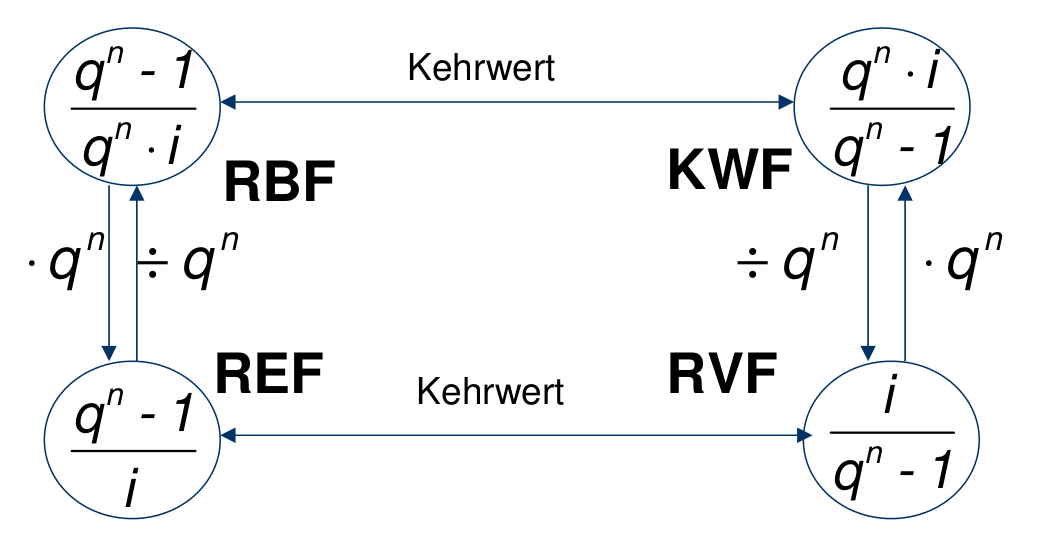
\includegraphics[height=4cm]{RentenUndKapitalfaktoren.png}
\end{center}

Dem Karnevalsverein B.W.L (Bochumer Weißwurst Liga) steht durch den Abbau seiner Niederlassung in Querenburg die Summe von 300'\euro \ zur Verfügung, die langfristig investiert werden soll. Dafür hat er folgende Optionen:
\begin{enumerate}
	\item Anheuern der talentierten Büttenrednerin Berta Wassermann. Diese erklärt sich bereit, für 200' \euro \ die nächsten 3 Jahre auf Prunksitzungen des Vereins aufzutreten. Der Verein erwartet dadurch zusätzliche Einnahmen von 120' \euro \ pro Jahr.
	\item Investition in Ü-Ei Sammelfiguren. Auf einer bekannten online Autionsbörse steht zur Zeit eine Sammlung von zehntausend Figuren im Gesammtwert von 220' \euro \ zum Verkauf. Diese generieren keinen Mehrwert, aber der Marketingleiter der B.W.L geht davon aus, die Figuren in 4 Jahren für 480' \euro \ verkaufen zu können.
	\item Anlage bei einer Bank. Da der Filialleiter auch gleichzeitig Prinz des Karnevalsumzugs ist, gibt es hier Zinsen von 10\%.
\end{enumerate}
Berechne den Kapitalwert der Anlagen. Für welche sollte sich B.W.L entscheiden?

\ifshowsolution
	\begin{description}
		\item[Anlage 1] $- 200' + 120' \cdot \frac{1.10^3 - 1}{1.10^3 \cdot 0.1} \approx 98.4222'$
		\item[Anlage 2] $- 220' + 480' \cdot \frac{1}{1.10^4} \approx 107.8465'$
		\item[Anlage 3] 0, weil Standardoption (Interner Zinsfuß oder so)
	\end{description}
	Der Verein sollte sich also für Anlage 2 entscheiden.
\fi

\subsection{Investitionsrechnung}
Helmut B. plant die Eröffnung einer Druckerei. Dafür ist die Anschaffung einer Buchpresse erforderlich. Nachdem er Angebote eingeholt hat, stehen folgende Pressen, die jeweils 5 Jahre genutzt werden sollen, in der engeren Auswahl:

\begin{tabular}{lrr}
	& Presse 1 & Presse 2 \\ \hline
	Anschaffungskosten (\euro) & 450.000 & 300.000 \\
	sonstige fixe Kosten (\euro) p.a. & 15.000 & 12.000 \\
	variable Kosten (\euro \ pro Verpackungseinheit) & 22 & 25 \\
	Restverkaufserlös (\euro) & 80.000 & 50.000
\end{tabular}

Herr B. geht davon aus, 14.000 Verpackungseinheiten mit jeweils 20 Büchern verkaufen zu können und rechnet mit 5\% Zinsen.

\begin{enumerate}
	\item Welche Presse ist nach Kostenvergleichsrechnung die bessere Wahl?
	
	\ifshowsolution
		\begin{tabular}{lr|r}
			Abschreibung & $\frac{450.000 - 80.000}{5} = 74.000$ & $\frac{300.000 - 50.000}{5} = 50.000$ \\
			Kalkulatorischer Zins & $\frac{450.000 + 80.000}{2} \cdot 0.05 = 13.250$ & $\frac{300.000 + 50.000}{2} \cdot 0.05 = 8.750$ \\
			Sonstige Fixkosten & 15.000 & 12.000 \\
			Variable Kosten & $14.000 \cdot 22 = 308.000$ & $14.000 \cdot 25 = 350.000$ \\ \hline
			$\sum$ & 410.250 & 420.750
		\end{tabular}
		
		Er sollte sich also für Presse 1 entscheiden.
	\fi
	
	\item Bei welcher Produktionsmenge an Verpackungseinheiten sind beide Pressen gleich gut?
	
	\ifshowsolution
		\begin{align*}
			\underbrace{410.250}_{\text{Kosten pro Jahr}} - \underbrace{308.000}_{\text{variable Kosten}} &= \underbrace{102.250}_{\text{Fixe Kosten}} \tag{Maschine 1} \\
			\underbrace{420.750}_{\text{Kosten pro Jahr}} - \underbrace{350.000}_{\text{variable Kosten}} &= \underbrace{70.750}_{\text{Fixe Kosten}} \tag{Maschine 2} \\
			\text{Fixkosten}_1 + \text{variable Kosten}_1 &\setequal \text{Fixkosten}_2 + \text{variable Kosten}_2 \\
			102.250 + 22 \cdot x &= 70.750 + 25 \cdot x \\
			x &= 10.500
		\end{align*}
	\fi
	
	\item Da Presse 1 zusätzlich noch das Gesicht des charmanten Herrn B. auf das Cover drucken kann, rechnet her hier mit einem Verkaufspreis von 18\euro \ je Buch, bei Presse 2 jedoch nur mit 16\euro \ je Buch. Für welche Presse entscheidet er sich nach einer Gewinnvergleichsrechnung? Wir nehmen dabei an, dass Presse 1 Kosten von 410.000 \euro \ und Presse 2 Kosten von 420.000 \euro \ verursacht (zur Vermeidung von Folgefehlern).
	
	\ifshowsolution
		\begin{tabular}{l|r|r}
			& Presse 1 & Presse 2 \\ \hline
			Erlös & $18 \cdot 20 \cdot 14.000 =5.040.000$ & $16 \cdot 20 \cdot 14.000 = 4.480.000$ \\
			Kosten & 410.000 & 420.000 \\ \hline
			Gewinn & 4.630.000 & 4.060.000
		\end{tabular}
		
		Presse 1 bietet einen höheren Gewinn, daher wird man sich für diese entscheiden.
	\fi
\end{enumerate}

\subsection{Äquivalenzziffernrechnung}
Der Lebensmittelhersteller Krafft vertreibt 4 Sorten Energy-Drinks. Die Kosten pro Palette ergeben sich zum Großteil aus der Herstellungsdauer. In der folgenden Tabelle sind die Herstellungszahlen und Produktionszeiten pro Palette und Typ angegeben. Die gesammten Herstellungskosten betragen 320.000 \euro.

\begin{tabular}{lcc}
	Energy-Drink & Produktionszahlen (in Paletten) & Hertellungsdauer (in Minuten) \\ \hline
	Ungehäuer & 2400 & 24 \\
	Blue Donkey & 1200 & 32 \\
	Rhinozeros & 600 & 18 \\
	Metalikone & 2000 & 20
\end{tabular}

Wie groß sind die Herstellungskosten in vollen Tausend \euro \ pro Produkttyp, wenn man die einstufige Äquivalenzziffernrechnung anwendet?

\ifshowsolution
	Da die Herstellungsdauer den Hauptanteil an den Kosten ausmacht, sind die die Kosten für einen Produkttyp proportional zur Herstellungsdauer pro Palette mal Anzahl der hergestellten Paletten. Diese rechnen wir zunächst aus ('Palettenminuten').

	Der Anteil der Kosten, den ein Produkttyp an den Gesammtkosten hat, entspricht nun dem Anteil der Palettenminuten an der Summe aller Palettenminuten. Diesen Anteil rechnen wir aus indem wir die Palettenminuten eines Produkttyps durch die Summe der Palettenminuten dividieren, das Ergebnis wird dann 'Äquivalenzziffer' genannt.

	Die Kosten, die auf einen Produkttyp entfallen, ergeben sich dann dadurch, dass wir die Gesammtkosten mit der jeweiligen Äquivalenzziffer multiplizieren.

	\begin{tabular}{lrrrrr}
		Energy-Drink & Paletten & Minuten & Palettenminuten & Äquivalenzziffer & Kosten \\ \hline
		Ungehäuer & 2400 & 24 & 57600 & 0.3924 & 125' \\
		Blue Donkey & 1200 & 32 & 38400 & 0.2616 & 83' \\
		Rhinozeros & 600 & 18 & 10800 & 0.0736 & 23' \\
		Metalikone & 2000 & 20 & 40000 & 0.2725 & 87' \\ \hline
		$\sum$ & & & 146800 & 1.0001 & 318'
	\end{tabular}
\fi

%%%%%%%%%%%%%%%%%%%%%%%%%%%%%%%%%%%%%%%%%%%%%%%%%%%%%%%%%%%%%%%%%%%%%%%%%%%%%%%%
%                                Sonstiges                                     %
%%%%%%%%%%%%%%%%%%%%%%%%%%%%%%%%%%%%%%%%%%%%%%%%%%%%%%%%%%%%%%%%%%%%%%%%%%%%%%%%
\newpage
\section{Sonstiges}
\subsection{Binäre Zahlen}
Welche Dezimalzahlen entsprechen den folgenden Binärzahlen?
\begin{enumerate}
	\item
		\ifshowsolution
			\begin{tabular}{l|l|l}
				110 & 1010 & 10001 \\ \hline
				$6_d$ & $10_d$ & $17_d$
			\end{tabular}
		\else
			\begin{tabular}{l|l|l}
				110 & 1010 & 10001 \\ \hline
				& &
			\end{tabular}
		\fi
	\item
		\ifshowsolution
			\begin{tabular}{l|l|l}
				11101 & 100100 & 1110001101 \\ \hline
				$29_d$ & $26_d$ & $909_d$
			\end{tabular}
		\else
			\begin{tabular}{l|l|l}
				11101 & 100100 & 1110001101 \\ \hline
				& &
			\end{tabular}
		\fi
\end{enumerate}

Schreibe folgende Dezimalzahlen im Binärsystem
\begin{enumerate}
	\item
		\ifshowsolution
			\begin{tabular}{l|l|l|l|l}
				1 & 2 & 4 & 8 & 16 \\ \hline
				$1_b$ & $10_b$ & $100_b$ & $1000_b$ & $10000_b$
			\end{tabular}
		\else
			\begin{tabular}{l|l|l|l|l}
				1 & 2 & 4 & 8 & 16 \\ \hline
				& & & &
			\end{tabular}
		\fi
	\item
		\ifshowsolution
			\begin{tabular}{l|l|l}
				3 & 7 & 15 \\ \hline
				$11_b$ & $111_b$ & $1111_b$
			\end{tabular}
		\else
			\begin{tabular}{l|l|l}
				3 & 7 & 15 \\ \hline
				& &
			\end{tabular}
		\fi
	\item
		\ifshowsolution
			\begin{tabular}{l|l|l|l}
				5 & 11 & 28 & 42\\ \hline
				$101_b$ & $1011_b$ & $11100_b$ & $101010_b$
			\end{tabular}
		\else
			\begin{tabular}{l|l|l|l}
				5 & 11 & 28 & 42\\ \hline
				& & &
			\end{tabular}
		\fi
\end{enumerate}
Führe folgende Berechnungen durch
\begin{enumerate}
	\item $1101_b + 110_b$
	
	\ifshowsolution
		$1101_b + 110_b = 10011_b$
	\fi
	
	\item $1011101_b + 1001_b$
	
	\ifshowsolution
		$1011101_b + 1001_b = 1100110_b$
	\fi
	
	\item $1011101_b - 1001_b$
	
	\ifshowsolution
		$1011101_b - 1001_b = 1010100_b$
	\fi
	
	\item $1101_b - 110_b$
	
	\ifshowsolution
		$1101_b - 110_b = 111_b$
	\fi
	
	\item $1101_b \cdot 110_b$
	
	\ifshowsolution
		$1101_b \cdot 110_b = 1001110_b$
	\fi
	
	\item $1011101_b \cdot 1001_b$
	
	\ifshowsolution
		$1011101_b \cdot 1001_b = 1101000101_b$
	\fi
\end{enumerate}

\subsection{Modulare Arithmetik}
Was ist das Ergebnis folgender Rechnungen?
\begin{enumerate}
	\item $3 \bmod 3$
	
	\ifshowsolution
		$3 \bmod 3 \equiv 0$
	\fi
	
	\item $7 \bmod 3$
	
	\ifshowsolution
		$7 \bmod 3 \equiv 1$
	\fi
	
	\item $13 \bmod 5$
	
	\ifshowsolution
		$13 \bmod 5 \equiv 3$
	\fi
	
\end{enumerate}
Zu welchem Wert sind die folgenden Terme äquivalent?
\begin{enumerate}
	\item $3 + 4 \pmod 2$
	
	\ifshowsolution
		$3 + 4 \pmod 2 \equiv 1$
	\fi
	
	\item $12 + 1 \pmod 5$
	
	\ifshowsolution
		$12 + 1 \pmod 5 \equiv 3$
	\fi
	
	\item $4 \cdot 5 \pmod 7$
	
	\ifshowsolution
		$4 \cdot 5 \pmod 7 \equiv 6$
	\fi
	
	\item $3 \cdot 8 \pmod {11}$
	
	\ifshowsolution
		$3 \cdot 8 \pmod {11} \equiv 2$
	\fi
	
\end{enumerate}
Welches x löst die Gleichung?
\begin{enumerate}
	\item $0 + x \equiv 3 \pmod 5$
	
	\ifshowsolution
		$x \equiv 3$
	\fi
	
	\item $1 + x \equiv 0 \pmod 5$
	
	\ifshowsolution
		$x \equiv 4$
	\fi
	
	\item $4 + x \equiv 2 \pmod 5$
	
	\ifshowsolution
		$x \equiv 3$
	\fi
\end{enumerate}

\end{document}









